\documentclass[a4paper]{article}

\def\npart {Bayesian Population PK}
\def\nterm {Inference reading notes}
\def\nyear {2026}
\def\nlecturer {MIT 6.008/6.437 and Marc Lavielle}
\def\ncourse {Population PK as Bayesian Inference}
\def\ncoursehead {Bayesian PopPK}
\def\nauthor {NanFangHong}

\RequirePackage{etex}
\makeatletter
\ifx \npart \undefined
  \def\npart{PK/PD Notes}
\fi
\ifx \nterm \undefined
  \def\nterm{Reading notes}
\fi
\ifx \nyear \undefined
  \def\nyear{\the\year}
\fi
\ifx \nlecturer \undefined
  \def\nlecturer{the source literature}
\fi
\ifx \nauthor \undefined
  \def\nauthor{NanFangHong}
\fi
\ifx \ncourse \undefined
  \def\ncourse{Pharmacology Reading Note}
\fi
\ifx \ncoursehead \undefined
  \def\ncoursehead{\ncourse}
\fi

\author{Based on \nlecturer \\\small Notes taken by \nauthor}
\date{\nterm\ \nyear}
\title{\npart\ --- \ncourse}

\usepackage{amsfonts}
\usepackage{amsmath}
\usepackage{amssymb}
\usepackage{amsthm}
\usepackage{booktabs}
\usepackage{caption}
\usepackage{enumitem}
\usepackage{fancyhdr}
\usepackage{fontspec}
\usepackage{graphicx}
\usepackage{iftex}
\usepackage{mathtools}
\usepackage{microtype}
\usepackage{siunitx}
\usepackage{tabularx}
\usepackage{tikz}
\usepackage{xcolor}
\usepackage{xurl}
\usepackage{xeCJK}

\IfFontExistsTF{Latin Modern Roman}{
  \setmainfont[Ligatures=NoCommon]{Latin Modern Roman}
}{}

\IfFontExistsTF{Noto Serif CJK SC}{
  \setCJKmainfont{Noto Serif CJK SC}
}{
  \IfFontExistsTF{Songti SC}{
    \setCJKmainfont{Songti SC}
  }{
    \IfFontExistsTF{PingFang SC}{
      \setCJKmainfont{PingFang SC}
    }{}
  }
}

\usepackage[hidelinks,unicode,breaklinks=true]{hyperref}
\hypersetup{
  pdfauthor={\nauthor},
  pdfsubject={\npart\ - \ncourse},
  pdftitle={\npart\ - \ncourse},
  pdfkeywords={PK PD pharmacology reading notes \ncourse}
}

\pagestyle{fancyplain}
\lhead{\emph{\nouppercase{\leftmark}}}
\rhead{
  \ifnum\thepage=1
  \else
    \npart\ \ncoursehead
  \fi}

\theoremstyle{definition}
\newtheorem*{aim}{Aim}
\newtheorem*{assumption}{Assumption}
\newtheorem*{defi}{Definition}
\newtheorem*{eg}{Example}
\newtheorem*{notation}{Notation}
\newtheorem*{question}{Question}
\newtheorem*{remark}{Remark}
\newtheorem*{warning}{Warning}

\theoremstyle{plain}
\newtheorem{nthm}{Theorem}[section]
\newtheorem{nprop}[nthm]{Proposition}

\renewcommand{\labelitemi}{--}
\renewcommand{\labelitemii}{$\circ$}
\renewcommand{\labelenumi}{(\roman{*})}

\let\stdsection\section
\renewcommand\section{\newpage\stdsection}

\newcommand{\dd}{\mathop{}\!\mathrm{d}}
\newcommand{\Emax}{E_{\max}}
\newcommand{\pksym}[1]{\ifmmode\text{\textit{#1}}\else\textit{#1}\fi}
\newcommand{\pklab}[1]{\mathrm{#1}}
\newcommand{\ECfifty}{\pksym{EC}_{50}}
\newcommand{\term}[1]{\emph{#1}}
\makeatother

\usetikzlibrary{fit,positioning}
\emergencystretch=2em
\title{Bayesian Population PK - Population PK as Bayesian Inference}

\DeclareMathOperator*{\argmax}{arg\,max}
\DeclareMathOperator*{\argmin}{arg\,min}
\DeclareMathOperator{\diag}{diag}
\DeclareMathOperator{\logit}{logit}
\newcommand{\rv}[1]{\mathsf{#1}}
\newcommand{\bs}[1]{\boldsymbol{#1}}
\newcommand{\given}{\,|\,}
\newcommand{\Prob}{\mathbb{P}}
\newcommand{\E}{\mathbb{E}}
\newcommand{\Var}{\operatorname{var}}
\newcommand{\Cov}{\operatorname{cov}}
\newcommand{\Normal}{\mathcal{N}}
\newcommand{\lik}{\mathcal{L}}
\newcommand{\data}{\mathcal{D}}
\newcommand{\R}{\mathbb{R}}
\newcommand{\iid}{\overset{\mathrm{iid}}{\sim}}
\newcommand{\indep}{\perp\!\!\!\perp}
\newcommand{\pop}{\mathrm{pop}}
\newcommand{\obs}{\mathrm{obs}}
\newcommand{\pred}{\mathrm{pred}}
\newcommand{\post}{\mathrm{post}}

\begin{document}
\maketitle
{\small
  \noindent\textbf{Reading motive}\\
  These notes connect the inference language of MIT 6.008/6.437 with Marc Lavielle's mixed effects population approach. The guiding claim is that Population PK is not a collection of software tricks; it is a pharmacological instance of hierarchical Bayesian inference.\hspace*{\fill}[inference]

  \vspace{5pt}
  \noindent\textbf{Audience}\\
  The intended reader has not taken 6.008/6.437 and has not used NONMEM. We begin with probability laws, conditioning, Bayes rule, and latent variables, then move gradually into \(\pklab{PK}\) ODEs, individual parameters, population distributions, marginal likelihood, SAEM, and NONMEM.\hspace*{\fill}[from zero]

  \vspace{5pt}
  \noindent\textbf{Style}\\
  This is a reconstruction rather than an excerpt. The notation borrows the 6.437 random-variable convention: random quantities use sans-serif symbols, while realizations and parameters use ordinary type. The Population PK structure follows Lavielle's \(y_i,\psi_i,\theta\) language.\hspace*{\fill}[notation]
}

\tableofcontents

\section{Source map and thesis}

\subsection{Three source streams}

我这里同时读三条线：

\begin{itemize}[leftmargin=2em]
  \item \textbf{MIT 6.008}: probability law、conditional probability、random variables、decision making、graphical models、model selection、asymptotics、Markov chains、sampling methods、continuous inference。它是 6.437 的地基，给出 ``how to think probabilistically'' 的起点 \cite{mit6008notes}。
  \item \textbf{MIT 6.437}: Bayesian hypothesis testing、Bayesian parameter estimation、non-Bayesian decision theory、exponential families、sufficient statistics、EM、information geometry、modeling as inference、MCMC、typicality、method of types、asymptotics 和 model selection。它不是另起炉灶，而是在 6.008 的 probability/inference grammar 上继续加深 \cite{mit6437notes}。
  \item \textbf{Lavielle}: mixed effects models for the population approach。它把这个 grammar 落到 pharmacometrics: observations \(y_i\)、individual parameters \(\psi_i\)、population parameters \(\theta\)、covariates \(c_i\)、and the joint model \cite{lavielle2015mixed}。
\end{itemize}

\begin{remark}
  读 Lavielle 最舒服的地方是，他很少把模型当成 ``software syntax''。他反复区分 description, mathematical representation, implementation。这个区分对 Population PK 特别重要：一个 one-compartment model 可以是 ODE，可以是 closed-form equation，也可以是 NONMEM 或 Mlxtran 代码；这些不是三种模型，而是同一个模型的不同表述。
\end{remark}

\subsection{The learning order}

这篇笔记必须按下面的顺序走：
\[
  \text{6.008}
  \longrightarrow
  \text{6.437}
  \longrightarrow
  \text{Lavielle}
  \longrightarrow
  \text{NONMEM/Monolix/SAEM}.
\]

\begin{warning}
  如果跳过 6.008，6.437 里的 posterior、risk、EM、typicality、model selection 会变成一串公式；如果跳过 6.437，Population PK 里的 likelihood、EBE、SAEM、posterior predictive check 又会像软件黑话。6.008 是语感，6.437 是深度，Lavielle 是落地。
\end{warning}

\subsection{The main thesis}

Population PK 的核心对象不是一条 concentration--time curve，而是一个条件概率系统：
\[
  p_\theta(y_i,\psi_i\given c_i,u_i)
  =
  p_\theta(y_i\given \psi_i,u_i)\,
  p_\theta(\psi_i\given c_i).
\]
这里
\begin{itemize}[leftmargin=2em]
  \item \(y_i\) 是第 \(i\) 个个体的观测数据，比如浓度、PCA、biomarker 或 categorical outcome；
  \item \(\psi_i\) 是这个个体自己的 PK/PD 参数，比如 \(\pksym{CL}_i,V_i,k_{a,i},\pksym{EC}_{50,i}\)；
  \item \(c_i\) 是 covariates，比如 weight、sex、genotype、renal function；
  \item \(u_i\) 是 design/dosing regimen，比如 dose、infusion、sampling times；
  \item \(\theta\) 是 population-level unknowns，比如 typical values、covariate effects、\(\Omega\)、residual error parameters。
\end{itemize}

The population approach says: we do not observe \(\psi_i\), but we can infer them by combining each individual's sparse data with the population distribution. 这句话已经是 Bayesian inference。

\subsection{Why this matters}

经典 individual PK 是：
\[
  \text{fit each subject separately} \quad \longrightarrow \quad
  \text{summarize the fitted parameters}.
\]
Population PK 是：
\[
  \text{learn the population distribution and individual posteriors together}.
\]
这两句话的差异非常大。前者在 sparse sampling 时会崩，因为每个人的数据不足以识别自己的参数。后者允许 borrowing strength: 一个个体的数据很少，但 population prior-like distribution 提供了约束。

\begin{question}
  Population PK 为什么不是 ``平均曲线拟合''？
\end{question}

因为 population curve 只是一个 summary。真正的对象是 variability: 谁偏离 typical subject，偏离多少，偏离能否由 covariates 解释，剩下的不确定性应该如何传播到 prediction 和 decision。

\section{6.008 first: probability as modeling}

\subsection{A probability law is a modeling choice}

6.008 的第一层不是 Bayes rule，而是更朴素的一句话：
\[
  \text{a probabilistic model is a sample space plus a probability law}.
\]
一个模型先定义哪些 outcomes 可能发生，再定义每个 event 的 probability。这个视角对 Population PK 很重要，因为 pharmacometric model 不是先从 ``拟合曲线'' 开始，而是先定义：如果这个模型是真的，什么样的数据会被生成？

For a single subject, the sample outcome is not just one number. It may be the whole longitudinal record:
\[
  y_i=(y_{i1},\ldots,y_{in_i}).
\]
If we also include unobserved individual parameters, a fuller outcome is
\[
  (y_i,\psi_i).
\]
Population modeling says that the sample space should be large enough to include both observed data and latent biological variability.

\begin{remark}
  6.008 喜欢问 sample space 的 granularity。PopPK 里同样如此：如果我们只关心 concentration，\(y_i\) 是 concentration vector；如果我们关心 PK/PD，\(y_i\) 可能有 concentration 和 response 两个 observation streams；如果 dropout is informative，event time 也必须成为 sample outcome 的一部分。
\end{remark}

\subsection{The right level of detail}

6.008 的 dice/image examples 都在强调同一件事：sample space 可以极大，关键是选对 granularity。Population PK 的 granularity 也有层级：

\begin{center}
\begin{tabularx}{0.96\textwidth}{p{0.24\textwidth}X}
\toprule
Granularity & PopPK version \\
\midrule
One observation & \(\rv{y}_{ij}\), a concentration at one time. \\
One individual & \(\rv{y}_i=(\rv{y}_{i1},\ldots,\rv{y}_{in_i})\), the longitudinal record. \\
One latent individual & \((\rv{y}_i,\rv{\psi}_i)\), observations plus the subject's hidden PK parameters. \\
The population sample & \((\rv{y}_{1:N},\rv{\psi}_{1:N})\), all individuals and all latent heterogeneity. \\
Future trial or clinic & \((\tilde{\rv{y}},\tilde{\rv{\psi}})\), prediction for new individuals. \\
\bottomrule
\end{tabularx}
\end{center}

The modeler must choose the sample space to match the scientific question. 如果目标是 estimating clearance variability，\(\psi_i\) 必须进入模型；如果目标是 deciding dose adjustment，future exposure \(\tilde y\) 必须进入 prediction。

\subsection{Events in PopPK}

6.008 讲 event 是 sample space 的 subset。药理学里的 event 往往就是临床问题：
\[
  A=\{\tilde C_{\min}<C_{\mathrm{target}}\},
\]
\[
  B=\{\pksym{AUC}_{0-24} > \pksym{AUC}_{\mathrm{tox}}\},
\]
\[
  G=\{\pksym{CL}_i \text{ is below the 10th population percentile}\}.
\]
一旦我们有 posterior predictive distribution，就可以计算
\[
  \Prob(A\given y_i)
  =
  \int 1\{\tilde C_{\min}<C_{\mathrm{target}}\}
  p(\tilde C_{\min}\given y_i)\,\dd \tilde C_{\min}.
\]
这就是从 probability law 到 clinical decision 的最短路径。

\section{6.008 conditioning: the first Bayes move}

\subsection{Conditional probability}

6.008 的 conditional probability 定义是
\[
  \Prob(A\given B)=\frac{\Prob(A\cap B)}{\Prob(B)}.
\]
它的直觉是：知道 \(B\) 发生后，我们把 sample space 缩到 \(B\)，再重新归一化。

PopPK 里 \(B\) 通常是 ``we observed this individual's data'':
\[
  B=\{\rv{y}_i=y_i\}.
\]
而 \(A\) 可能是 ``this individual has low clearance'':
\[
  A=\{\rv{CL}_i < 0.6\,\pksym{CL}_{\pop}\}.
\]
于是
\[
  \Prob(\rv{CL}_i < 0.6\,\pksym{CL}_{\pop}\given \rv{y}_i=y_i)
\]
就是一个 individual-level posterior probability。

\subsection{Law of total probability}

Bayes rule 之前还有一个更 foundational 的式子：law of total probability。若 \(\psi_i\) 是 latent parameter，
\[
  p_\theta(y_i)
  =
  \int
  p_\theta(y_i\given \psi_i)
  p_\theta(\psi_i)
  \dd\psi_i.
\]
这就是 observed-data likelihood for one individual。看起来像 Population PK 的高级公式，其实只是 6.008 的 total probability applied to a latent continuous variable。

\begin{remark}
  所以 Population PK 的核心积分不是从 pharmacometrics 天上掉下来的。它就是 ``把没有观察到的 individual parameters 加总/积分掉''。
\end{remark}

\subsection{Bayes rule as reweighting}

Bayes rule:
\[
  p_\theta(\psi_i\given y_i)
  =
  \frac{
    p_\theta(y_i\given \psi_i)p_\theta(\psi_i)
  }{
    \int p_\theta(y_i\given \psi_i)p_\theta(\psi_i)\,\dd\psi_i
  }.
\]
It says: start with population plausibility \(p_\theta(\psi_i)\), reweight each \(\psi_i\) by how well it predicts the observed data \(p_\theta(y_i\given\psi_i)\), then normalize.

这个 reweighting image 比 ``Bayes theorem'' 这个词更重要：
\[
  \text{posterior}
  \propto
  \text{likelihood}
  \times
  \text{population distribution}.
\]

\section{6.008 random variables}

\subsection{Random variables are functions of outcomes}

6.008 里的 random variable 不是玄学对象，而是 outcome 的函数。对 PopPK 来说，一个 complete outcome 可能包含 whole concentration curve and latent physiology。Random variables are summaries of that outcome:
\[
  \rv{CL}_i,\quad \rv{V}_i,\quad \rv{AUC}_i,\quad
  \rv{C}_{\max,i},\quad \rv{T}_{>\pklab{MIC},i}.
\]
Once a probability law is assigned, these summaries inherit distributions.

例如若 \(\pksym{CL}_i\) 是 log-normal:
\[
  \log \rv{CL}_i\sim \Normal(\log \pksym{CL}_{\pop},\omega_{\pklab{CL}}^2),
\]
那么 \(\pksym{AUC}_i=D/\rv{CL}_i\) 也有 induced distribution。This is why parameter uncertainty automatically becomes exposure uncertainty.

\subsection{Expectation}

Expectation in 6.008 is a weighted average:
\[
  \E[g(\rv{x})]=\sum_x g(x)p(x)
  \quad \text{or} \quad
  \E[g(\rv{x})]=\int g(x)p(x)\,\dd x.
\]
In PopPK:
\[
  \E[\rv{CL}_i\given y_i]
  =
  \int \pksym{CL}_i\,p(\pksym{CL}_i\given y_i)\,\dd \pksym{CL}_i.
\]
This posterior mean is an estimator under squared-error loss. It is not necessarily the same as MAP/EBE:
\[
  \widehat{\pksym{CL}}^{\pklab{MAP}}_i
  =
  \argmax_{\pksym{CL}_i}p(\pksym{CL}_i\given y_i).
\]

\subsection{Independence and conditional independence}

6.008 distinguishes independence:
\[
  \rv{x}\indep \rv{z}
\]
from conditional independence:
\[
  \rv{x}\indep \rv{z}\given \rv{w}.
\]
Population PK lives on conditional independence. Given individual parameters, observations are often assumed independent:
\[
  \rv{y}_{ij}\indep \rv{y}_{ik}\given \rv{\psi}_i
  \quad (j\ne k).
\]
Given population parameters, individuals are often assumed independent:
\[
  (\rv{y}_i,\rv{\psi}_i)
  \indep
  (\rv{y}_l,\rv{\psi}_l)
  \given \theta
  \quad (i\ne l).
\]
These assumptions are not automatic truth. They are modeling commitments. Carryover, adherence, informative dropout, shared batch effects, or site effects can break them.

\section{6.008 decision making: estimates are decisions}

\subsection{Loss functions}

6.008 的 decision-making framework 很适合纠正一个常见误解：estimate is not truth; estimate is a decision. To choose an estimate, we first choose a loss.

For a posterior \(p(\psi_i\given y_i)\):
\[
  \widehat{\psi}(y_i)
  =
  \argmin_a
  \E\{C(\rv{\psi}_i,a)\given y_i\}.
\]
Different losses give different summaries:

\begin{center}
\begin{tabularx}{0.96\textwidth}{p{0.25\textwidth}X}
\toprule
Loss & Estimator \\
\midrule
0--1 or small-ball loss & MAP / posterior mode. \\
Squared error & Posterior mean. \\
Absolute error & Posterior median. \\
Asymmetric clinical loss & A threshold-aware decision, not a standard summary. \\
\bottomrule
\end{tabularx}
\end{center}

\subsection{Why this matters for dosing}

Suppose we estimate exposure and choose dose. Under-dosing and over-dosing are not symmetric. A loss might be
\[
  C(\pksym{AUC},\widehat{\pksym{AUC}})
  =
  c_1\,1\{\pksym{AUC}<\pksym{AUC}_{\mathrm{eff}}\}
  +
  c_2\,1\{\pksym{AUC}>\pksym{AUC}_{\mathrm{tox}}\},
\]
where \(c_2\) may be much larger than \(c_1\) for a toxic drug. Then the optimal decision is not simply posterior mean exposure; it is a risk-minimizing action under the clinical loss.

\begin{remark}
  This is the hidden bridge from Bayesian inference to therapeutic drug monitoring: posterior predictive distributions matter because clinical action is a decision under asymmetric risk.
\end{remark}

\subsection{Soft versus hard}

6.008 calls probabilities soft information and decisions hard. A PopPK report often gives hard numbers:
\[
  \widehat{\pksym{CL}}_i=4.1\,\mathrm{L/h}.
\]
But what we actually know is softer:
\[
  p(\pksym{CL}_i\given y_i).
\]
If the posterior is wide or skewed, reporting only \(\widehat{\pksym{CL}}_i\) hides information that may matter more than the point estimate.

\section{6.008 graphical models: structure makes inference possible}

\subsection{Factorization}

6.008 uses graphical models to turn independence assumptions into factorization. For a tree model:
\[
  p(x_{1:n})=p(x_r)\prod_{(i,j)}p(x_j\given x_i).
\]
For PopPK:
\[
  p_\theta(y_{1:N},\psi_{1:N})
  =
  \prod_{i=1}^N
  p_\theta(\psi_i)
  p_\theta(y_i\given \psi_i).
\]
This factorization is why inference scales by individual. Without it, a joint distribution over all observations would be impossible to manipulate.

\subsection{The plate idea}

The ``plate'' around individuals means repeat this structure \(N\) times:
\[
  \theta
  \rightarrow
  \rv{\psi}_i
  \rightarrow
  \rv{y}_{ij}.
\]
The population parameters \(\theta\) are shared; individual parameters \(\psi_i\) are local; observations \(y_{ij}\) are even more local.

\begin{center}
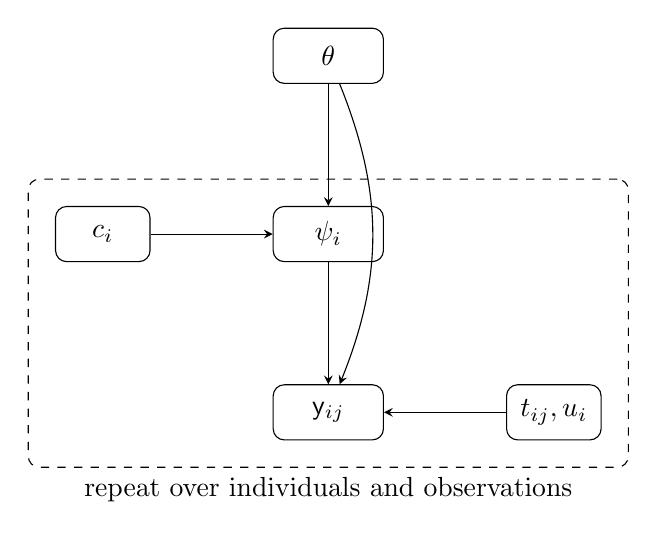
\begin{tikzpicture}[>=stealth, node distance=1.55cm, every node/.style={align=center}]
  \node[draw, rounded corners, minimum width=1.4cm, minimum height=0.7cm] (theta) {\(\theta\)};
  \node[draw, rounded corners, below=of theta, minimum width=1.4cm, minimum height=0.7cm] (psi) {\(\rv{\psi}_i\)};
  \node[draw, rounded corners, below=of psi, minimum width=1.4cm, minimum height=0.7cm] (y) {\(\rv{y}_{ij}\)};
  \node[draw, rounded corners, left=of psi, minimum width=1.2cm, minimum height=0.7cm] (c) {\(c_i\)};
  \node[draw, rounded corners, right=of y, minimum width=1.2cm, minimum height=0.7cm] (t) {\(t_{ij},u_i\)};
  \draw[->] (theta) -- (psi);
  \draw[->] (psi) -- (y);
  \draw[->] (c) -- (psi);
  \draw[->] (t) -- (y);
  \draw[->] (theta) to[bend left=22] (y);
  \node[draw, dashed, rounded corners, fit=(psi)(y)(c)(t), inner sep=0.34cm, label=below:{repeat over individuals and observations}] {};
\end{tikzpicture}
\captionof{figure}{The 6.008 graphical model idea applied to Population PK.}
\end{center}

\subsection{When the graph is wrong}

The graph encodes assumptions. If two subjects are from the same clinical site, they may share site-level effects. If samples are processed in the same assay batch, residual errors may be correlated. If dropout depends on unobserved disease state, missingness is informative. Then the graph needs more nodes:
\[
  \text{site},\quad \text{batch},\quad \text{dropout process},\quad \text{adherence}.
\]
Good model criticism often means asking which missing node would explain the residual pattern.

\section{6.008 sampling and asymptotics}

\subsection{Monte Carlo expectations}

6.008's Monte Carlo chapter begins with
\[
  \mu = \E[g(\rv{x})],
  \qquad
  \widehat\mu_K=\frac{1}{K}\sum_{k=1}^K g(x^{(k)}),
\]
where \(x^{(k)}\sim p(x)\). PopPK needs this constantly:
\[
  \E[g(\rv{\psi}_i)\given y_i]
  \approx
  \frac{1}{K}\sum_{k=1}^K g(\psi_i^{(k)}),
  \qquad
  \psi_i^{(k)}\sim p(\psi_i\given y_i).
\]
This is the conceptual ancestor of posterior simulation, importance sampling, MCMC, and predictive checks.

\subsection{Sampling future subjects}

A population model can simulate future individuals:
\[
  \tilde\psi \sim p_{\widehat\theta}(\psi\given \tilde c),
  \qquad
  \tilde y\sim p_{\widehat\theta}(y\given \tilde\psi,\tilde u).
\]
This two-step simulation is exactly what VPC-like thinking requires. It is also the cleanest way to teach what \(\Omega\) means: not a nuisance variance, but a generator of plausible biological diversity.

\subsection{Asymptotics as comfort, not a crutch}

6.008 introduces law of large numbers and asymptotic thinking. Population ML relies on similar comfort: as \(N\) grows, \(\widehat\theta\) may become consistent and approximately normal under regularity conditions. But pharmacometric datasets are often small, unbalanced, censored, and nonlinear. Therefore asymptotics should guide intuition, not replace diagnostics.

\section{6.008 model selection as an entry point}

\subsection{Models are approximations}

6.008 already makes model selection a practical issue: multiple probability laws can explain data at different levels of granularity. PopPK model selection asks:
\[
  \mathcal{M}_1:\ \text{one compartment}
  \quad \text{versus} \quad
  \mathcal{M}_2:\ \text{two compartments},
\]
\[
  \mathcal{M}_3:\ \pksym{CL}_i \text{ has weight effect}
  \quad \text{versus} \quad
  \mathcal{M}_4:\ \pksym{CL}_i \text{ has weight and renal effect}.
\]

Each model is a candidate probability law:
\[
  p_{\theta_m}^{(m)}(y).
\]
The goal is not to find ``the true model'' in a metaphysical sense. The goal is to find a model useful enough for explanation, prediction, and decision.

\subsection{Why this sets up 6.437}

6.008 gives the question:
\[
  \text{Which probability law should we use?}
\]
6.437 deepens it:
\[
  \text{What is the information loss if we use } q(y) \text{ instead of } p(y)?
\]
This is why the learning order matters. 6.008 teaches the objects; 6.437 teaches the geometry and decision theory of those objects.

\section{6.437 on top of 6.008}

\subsection{What gets added}

Once 6.008 gives us probability, conditioning, decision, graph, and sampling, 6.437 adds several layers:

\begin{itemize}[leftmargin=2em]
  \item Bayesian hypothesis testing: posterior odds, likelihood ratios, Bayes risk.
  \item Bayesian estimation: posterior mean, median, MAP, and loss-dependent estimators.
  \item Non-Bayesian decision theory: minimax, Neyman--Pearson, error exponents.
  \item Exponential families: sufficient statistics and data compression.
  \item EM: how to estimate parameters with latent complete data.
  \item Information geometry and modeling as inference: models as approximations measured by divergence.
  \item MCMC and typicality: why sampling can make high-dimensional inference practical.
\end{itemize}

Population PK borrows from all of these, but the most immediate bridges are Bayesian estimation, EM/SAEM, information-based model comparison, and posterior predictive thinking.

\subsection{How to read the rest}

From here onward, every PopPK concept should be read through a two-layer lens:
\[
  \text{6.008 asks: what probability law did we define?}
\]
\[
  \text{6.437 asks: what inference or decision are we performing with it?}
\]

\section{6.437 Bayesian hypothesis testing}

\subsection{Hypotheses as random variables}

6.437 begins Bayesian hypothesis testing by turning the unknown hypothesis into a random variable:
\[
  \rv{H}\in\{H_0,H_1,\ldots,H_{M-1}\}.
\]
The model is
\[
  p_{\rv{H}}(H_m),\qquad
  p_{\rv{y}\given \rv{H}}(y\given H_m).
\]
After observing \(y\), belief updates to
\[
  p_{\rv{H}\given \rv{y}}(H_m\given y)
  =
  \frac{
    p_{\rv{y}\given \rv{H}}(y\given H_m)
    p_{\rv{H}}(H_m)
  }{
    \sum_{\ell}
    p_{\rv{y}\given \rv{H}}(y\given H_\ell)
    p_{\rv{H}}(H_\ell)
  }.
\]

PopPK translation:
\[
  H_0:\ \text{one-compartment PK},
  \qquad
  H_1:\ \text{two-compartment PK}.
\]
or
\[
  H_0:\ \text{no renal covariate effect on }\pksym{CL},
  \qquad
  H_1:\ \text{renal function modifies }\pksym{CL}.
\]
In classical pharmacometrics, these are often compared by likelihood ratio, AIC/BIC, or OFV drop. In Bayesian workflows, we can compare posterior model probabilities or predictive performance.

\subsection{Likelihood ratio as evidence}

For two hypotheses, the posterior odds are
\[
  \frac{p(H_1\given y)}{p(H_0\given y)}
  =
  \frac{p(y\given H_1)}{p(y\given H_0)}
  \frac{p(H_1)}{p(H_0)}.
\]
The first ratio is the likelihood ratio, or Bayes factor if both \(p(y\given H_m)\) are fully integrated over parameters:
\[
  \pklab{BF}_{10}
  =
  \frac{p(y\given H_1)}{p(y\given H_0)}.
\]
This gives a clean reading of model comparison:
\[
  \text{posterior odds}
  =
  \text{data evidence}
  \times
  \text{prior odds}.
\]

\begin{remark}
  NONMEM's objective-function difference is not automatically a Bayes factor. It usually compares maximized or approximated likelihoods, not fully integrated model evidence.

  The inferential intuition is still related: how much better does one model explain the observed data after accounting for its structure?
\end{remark}

\subsection{Decision costs}

6.437 emphasizes costs \(C_{ij}\): the cost of deciding \(H_i\) when \(H_j\) is true. In PopPK model selection, costs are not symmetric:

\begin{itemize}[leftmargin=2em]
  \item choosing an over-complicated model may harm interpretability and extrapolation;
  \item choosing an under-complicated model may miss clinically important covariate effects;
  \item choosing a mechanistically wrong model may give bad trial simulations even if fit is acceptable.
\end{itemize}

Therefore model choice is not just maximizing likelihood. It is a decision under scientific and clinical loss.

\section{6.437 Bayesian parameter estimation}

\subsection{Posterior as the sufficient belief}

6.437's Bayesian parameter estimation says:
\[
  p(x\given y)
  =
  \frac{p(y\given x)p(x)}
  {\int p(y\given x')p(x')\,\dd x'}.
\]
The key theorem-like idea is not a theorem but a discipline:

\begin{quote}
  Once the posterior is known, every Bayesian estimator for every loss can be computed from it.
\end{quote}

For PopPK:
\[
  p(\psi_i\given y_i,\widehat\theta)
\]
is the belief about an individual parameter; different summaries are different decisions.

\subsection{MAP, mean, median}

Under posterior \(p(\psi_i\given y_i)\):
\[
  \widehat{\psi}^{\pklab{MAP}}_i
  =
  \argmax_{\psi_i}p(\psi_i\given y_i),
\]
\[
  \widehat{\psi}^{mean}_i
  =
  \int \psi_i p(\psi_i\given y_i)\,\dd \psi_i,
\]
\[
  \widehat{\psi}^{median}_i
  \text{ solves }
  \Prob(\rv{\psi}_i\le \widehat{\psi}^{median}_i\given y_i)=\frac{1}{2}.
\]
For skewed log-normal-like posteriors, these can differ substantially.

\begin{warning}
  When software prints one individual estimate, ask which estimator it is. A conditional mode, a conditional mean, and a post hoc fit are not the same inferential object.
\end{warning}

\subsection{Posterior predictive distribution}

The posterior for \(\psi_i\) is still not the final clinical object. Often we want future concentration:
\[
  p(\tilde y_i\given y_i)
  =
  \int
  p(\tilde y_i\given \psi_i)
  p(\psi_i\given y_i)
  \dd\psi_i.
\]
If the future question is dose adjustment, the design \(u_i\) changes:
\[
  p(\tilde y_i\given y_i,u_i^{new})
  =
  \int
  p(\tilde y_i\given \psi_i,u_i^{new})
  p(\psi_i\given y_i,u_i^{old})
  \dd\psi_i.
\]
This is the exact conceptual form behind individualized Bayesian forecasting.

\section{6.437 exponential families}

\subsection{Why exponential families matter}

6.437 spends time on exponential families because they clarify when data can be compressed without losing information about parameters. A canonical form is
\[
  p(z;\theta)
  =
  \exp\{\theta^T T(z)-A(\theta)+B(z)\}.
\]
Here \(T(z)\) is the sufficient statistic.

If complete data \(z\) were observed, estimation can often be driven by \(T(z)\). In PopPK, complete data would include latent individual parameters:
\[
  z=(y,\psi).
\]
For Gaussian random effects, sufficient-statistic-like objects include
\[
  \sum_i \eta_i,\qquad
  \sum_i \eta_i\eta_i^T.
\]
For residual errors, they include sums of squared residuals. This is precisely why EM/SAEM can work: it tries to replace missing sufficient statistics by conditional expectations or stochastic approximations.

\subsection{A Gaussian random-effects example}

Suppose
\[
  \rv{\eta}_i\sim \Normal(0,\Omega),
  \qquad
  h(\rv{\psi}_i)=\mu+B c_i+\rv{\eta}_i.
\]
If \(\eta_i\) were observed, \(\Omega\) would be estimated from empirical covariance:
\[
  \widehat\Omega
  =
  \frac{1}{N}\sum_{i=1}^N \eta_i\eta_i^T.
\]
But \(\eta_i\) is hidden. EM-style algorithms replace this by
\[
  \frac{1}{N}\sum_i
  \E_{\theta^{(k)}}[
    \rv{\eta}_i\rv{\eta}_i^T
    \given y_i
  ].
\]
SAEM approximates this expectation by simulated conditional random effects and stochastic averaging.

\section{6.437 EM as a lower-bound idea}

\subsection{Observed likelihood is hard because of marginalization}

For incomplete data,
\[
  p_\theta(y)=\int p_\theta(y,z)\,\dd z.
\]
The log-likelihood
\[
  \log p_\theta(y)=\log\int p_\theta(y,z)\,\dd z
\]
is difficult because log and integral do not separate. EM avoids direct attack by using a current conditional distribution over missing data.

\subsection{The \(Q\)-function}

Define
\[
  Q(\theta\given\theta^{(k)})
  =
  \E_{\theta^{(k)}}[
    \log p_\theta(y,\rv{z})
    \given y
  ].
\]
Then EM maximizes \(Q\) repeatedly. Intuitively:

\begin{quote}
  Guess the hidden complete data distribution using the current model.
  Then fit the complete data model under that guess.
\end{quote}

In PopPK, \(z\) is \(\psi_{1:N}\), the collection of individual parameters.

\subsection{Why EM increases likelihood}

6.437 derives EM using a decomposition based on conditional distributions and Gibbs' inequality. A compact way to remember it:
\[
  \log p_\theta(y)
  =
  \mathcal{F}(q,\theta)
  +
  D\!\left(q(z)\,\|\,p_\theta(z\given y)\right),
\]
where \(\mathcal{F}\) is a lower bound. Setting
\[
  q(z)=p_{\theta^{(k)}}(z\given y)
\]
makes the bound tight at \(\theta^{(k)}\). Increasing the bound increases the observed likelihood, at least locally.

\begin{remark}
  This lower-bound view is the conceptual bridge to variational inference. SAEM is a different bridge: instead of deterministic lower-bound optimization, it simulates from the conditional latent distribution and uses stochastic approximation.
\end{remark}

\section{6.437 MCMC, typicality, and high dimension}

\subsection{Why high dimension is strange}

6.437's typicality material warns that high-dimensional probability does not behave like low-dimensional geometry. Most posterior mass may live in a shell rather than at the mode. This matters for PopPK because the latent vector
\[
  \psi_{1:N}=(\psi_1,\ldots,\psi_N)
\]
can be high-dimensional. A joint MAP may not represent a typical posterior draw.

\subsection{MCMC as dependent Monte Carlo}

When direct sampling is hard, MCMC builds a Markov chain
\[
  \psi^{(1)},\psi^{(2)},\ldots
\]
whose stationary distribution is the target posterior:
\[
  \pi(\psi)=p(\psi\given y).
\]
Then expectations are approximated by chain averages:
\[
  \E[g(\rv{\psi})\given y]
  \approx
  \frac{1}{K}\sum_{k=1}^K g(\psi^{(k)}).
\]
SAEM often uses MCMC-like simulation steps for individual parameters. Full Bayesian PopPK uses MCMC to sample both \(\theta\) and \(\psi_{1:N}\).

\subsection{Typicality and model checking}

A posterior predictive check asks whether observed data look typical under the fitted model:
\[
  \tilde y^{(k)}\sim p(\tilde y\given y),
  \qquad
  T(\tilde y^{(k)}) \text{ compared with } T(y).
\]
The statistic \(T\) might be peak concentration, trough, quantile over time, residual pattern, or dropout rate. This is typicality thinking translated into pharmacometrics.

\section{The 6.437 notation discipline}

\subsection{Random variable versus realization}

6.437 的一个很美的符号习惯是：random variables 用 sans-serif，比如 \(\rv{x}\)；具体实现值或 deterministic parameters 用 serif，比如 \(x\)。我在这篇笔记里采用这个区分：
\[
  \begin{aligned}
    \rv{y}_i &\quad \text{is random data},\\
    y_i &\quad \text{is the observed dataset}.
  \end{aligned}
\]
同理，
\[
  \begin{aligned}
    \rv{\psi}_i &\quad \text{is the latent individual parameter},\\
    \psi_i &\quad \text{is a candidate value of that parameter}.
  \end{aligned}
\]

\begin{notation}
  我会把 random quantities 写成 \(\rv{y},\rv{\psi},\rv{\eta}\)，把 realized data 和 deterministic parameters 写成 \(y,\psi,\eta,\theta\)。Population parameters \(\theta\) 在 maximum likelihood 或 empirical Bayes 语境下是 deterministic-but-unknown；在 full Bayesian 语境下也可以进一步建模为 random variable \(\rv{\theta}\)。
\end{notation}

\subsection{Probability laws}

6.008 从 sample space \(\Omega\) 和 probability law \(\Prob\) 开始。对 Population PK 来说，我们可以不用显式列出 \(\Omega\)，但必须知道每个模型声明都在定义一个 probability law。

例如一个观察模型
\[
  \rv{y}_{ij}\given \rv{\psi}_i=\psi_i
  \sim
  \Normal\!\left(f(t_{ij};\psi_i,u_i),\,\sigma^2\right)
\]
不是一句拟合口号，而是在定义 conditional density:
\[
  p_\theta(y_{ij}\given \psi_i,u_i)
  =
  \frac{1}{\sqrt{2\pi\sigma^2}}
  \exp\left\{
    -\frac{\{y_{ij}-f(t_{ij};\psi_i,u_i)\}^2}{2\sigma^2}
  \right\}.
\]

\subsection{Conditioning is information update}

Bayesian inference 的基本句式是：
\[
  p(x\given y)
  =
  \frac{p(y\given x)p(x)}{p(y)}.
\]
Population PK 里它变成：
\[
  p_\theta(\psi_i\given y_i,c_i,u_i)
  =
  \frac{
    p_\theta(y_i\given \psi_i,u_i)p_\theta(\psi_i\given c_i)
  }{
    \int p_\theta(y_i\given \psi_i,u_i)p_\theta(\psi_i\given c_i)\,\dd\psi_i
  }.
\]
这就是 individual posterior。NONMEM 里常说的 EBE 或 empirical Bayes estimate，就是这个 posterior 的某个 point summary，通常接近 posterior mode。

\begin{remark}
  这里的 ``prior'' 不是主观信念意义上的 prior，而是 population distribution。对第 \(i\) 个 individual 来说，它在数学上扮演 prior 的角色：还没有看见 \(y_i\) 之前，\(\psi_i\) 的 plausible range 由 \(p_\theta(\psi_i\given c_i)\) 决定。
\end{remark}

\section{Decision theory before software}

\subsection{Soft information and hard decisions}

6.008/6.437 反复提醒：posterior distribution 是 soft information，而 estimate 是 hard decision。Population PK 里也一样。

给定 posterior \(p_\theta(\psi_i\given y_i)\)，我们可以有不同 hard summaries:
\[
  \widehat{\psi}^{\pklab{MAP}}_i
  =
  \argmax_{\psi_i}
  p_\theta(\psi_i\given y_i),
\]
\[
  \widehat{\psi}^{\pklab{MMSE}}_i
  =
  \E_\theta[\rv{\psi}_i\given y_i],
\]
或者 posterior median、credible interval、posterior predictive distribution。不同 summary 对应不同 loss function。

\begin{warning}
  一个 EBE 不是 ``真实 individual parameter''。它是 posterior belief 在某个 loss function 下压成一个点的结果。Data sparse 时，posterior 会被 population distribution 拉回 typical value，这就是 shrinkage。
\end{warning}

\subsection{Risk, utility, and pharmacology}

6.008 的 decision-making 语言可以直接翻译成 pharmacometrics:

\begin{center}
\begin{tabularx}{0.96\textwidth}{p{0.28\textwidth}X}
\toprule
Inference object & Pharmacometric decision \\
\midrule
Posterior over \(\psi_i\) & 这个病人的 \(\pksym{CL}_i,V_i\) 可能是多少？\\
Posterior predictive \(p(\tilde y_i\given y_i)\) & 下一次 trough concentration 会不会低于目标？\\
Loss function \(C(a,\widehat a)\) & 低估 exposure 与高估 exposure 的临床代价是否对称？\\
Decision rule \(\delta(y)\) & 是否调剂量、是否加采样点、是否换模型？\\
\bottomrule
\end{tabularx}
\end{center}

这解释了为什么 Bayesian view 对 pharmacology 很自然：临床建模最终不是为了得到漂亮参数，而是为了在 uncertainty 下做 decision。

\section{From PK equations to random variables}

\subsection{A one-compartment structural model}

先忘掉 population。一个最小 oral one-compartment PK model 可以写成
\[
  \frac{\dd A_g(t)}{\dd t} = -k_a A_g(t),
\]
\[
  \frac{\dd A_c(t)}{\dd t}
  =
  F k_a A_g(t) - \frac{\pksym{CL}}{V}A_c(t),
  \qquad
  C(t)=\frac{A_c(t)}{V}.
\]
这里 \(A_g\) 是 gut/depot amount，\(A_c\) 是 central amount，\(C(t)\) 是 plasma concentration。The structural model \(f\) maps design and parameters to a prediction:
\[
  C(t;\psi,u)=f(t;\psi,u), \qquad
  \psi=(\pksym{CL},V,k_a,F).
\]

\begin{remark}
  Lavielle 的 Appendix C 强调：PK compartment model 是 ADME 的简化。它不是身体的真实地图，而是一个 quantitative approximation: enough structure to predict concentrations and enough simplicity to estimate parameters.
\end{remark}

\subsection{Observation model}

真实实验里我们不直接观察 \(f(t;\psi,u)\)，而是观察带误差的浓度：
\[
  \rv{y}_{ij}
  =
  f(t_{ij};\psi_i,u_i)
  +
  g(t_{ij};\psi_i,\xi)\rv{\epsilon}_{ij},
  \qquad
  \rv{\epsilon}_{ij}\iid \Normal(0,1).
\]
常见 residual error choices:
\[
  g = a \quad \text{constant error},
\]
\[
  g = b f(t_{ij};\psi_i,u_i) \quad \text{proportional error},
\]
\[
  g = a + b f(t_{ij};\psi_i,u_i) \quad \text{combined error}.
\]

这些不是 purely technical choices。它们表达测量误差如何随浓度变化。低浓度 assay noise 可能接近 constant；高浓度时 coefficient of variation 可能更稳定，proportional error 更自然。

\subsection{Why nonlinear matters}

如果 \(f\) 是 linear in parameters，mixed effects theory 会比较舒服。但 PK model 通常 nonlinear: \(\pksym{CL}/V\) 在指数里，\(k_a\) 和 \(\pksym{CL}/V\) 可能接近，\(F\) 与 \(V\) 可能缠在一起。于是
\[
  \int p_\theta(y_i\given \psi_i)p_\theta(\psi_i)\,\dd\psi_i
\]
通常没有 closed form。Population PK 的算法困难几乎都从这里开始。

\section{Individual parameters as latent variables}

\subsection{The Lavielle layer}

Lavielle 的 population approach 可以读成：
\[
  \rv{\psi}_i \sim p_\theta(\psi\given c_i),
  \qquad
  \rv{y}_i\given \rv{\psi}_i=\psi_i \sim p_\theta(y\given \psi_i,u_i).
\]
第一层描述 inter-individual variability；第二层描述 observation variability。

对正值参数，常用 log-normal model:
\[
  \log \rv{CL}_i
  =
  \log \pksym{CL}_{\pop} + \beta_{\pklab{CL}}^{\pklab{WT}}\log\!\left(\frac{\pksym{WT}_i}{70}\right)
  +
  \rv{\eta}_{\pklab{CL},i},
\]
\[
  \rv{\eta}_{\pklab{CL},i}\sim \Normal(0,\omega_{\pklab{CL}}^2).
\]
更紧凑地写：
\[
  h(\rv{\psi}_i)
  =
  \mu + B c_i + \rv{\eta}_i,
  \qquad
  \rv{\eta}_i\sim \Normal(0,\Omega).
\]
其中 \(h\) 可以是 log, logit, probit, identity 等 transformation。

\subsection{Typical value and variability}

一个 population parameter model 同时做两件事：

\begin{itemize}[leftmargin=2em]
  \item 给定 covariates \(c_i\)，定义 typical individual:
  \[
    \widetilde\psi_i = h^{-1}(\mu+Bc_i).
  \]
  \item 定义围绕 typical individual 的 unexplained variability:
  \[
    h(\rv{\psi}_i)-h(\widetilde\psi_i)=\rv{\eta}_i.
  \]
\end{itemize}

这就是 covariate modeling 的 inference meaning。Covariates 不是为了让表格好看，而是为了把一部分 variability 从 random unexplained bucket 移到 explainable structure。

\begin{question}
  如果加入 weight effect 后 \(\omega_{\pklab{CL}}\) 下降，这是否说明 weight ``causes'' clearance variability？
\end{question}

统计上更谨慎的说法是：weight explains part of the observed between-subject variation under this model class。因果解释还需要设计、机制、外部知识和 counterfactual reasoning。

\subsection{Shrinkage from sparse data}

假设某个 subject 只有两个 concentration samples。单独拟合 \(\pksym{CL}_i,V_i,k_{a,i}\) 几乎不可能。但在 population model 下，我们可以把信息分成两部分：
\[
  \log p_\theta(\psi_i\given y_i)
  =
  \log p_\theta(y_i\given \psi_i)
  +
  \log p_\theta(\psi_i\given c_i)
  -
  \log p_\theta(y_i).
\]
第一项是 individual data support；第二项是 population support。数据少时，第二项更强，EBE 会向 typical value 收缩。这不是算法缺陷，而是 Bayesian updating 的必然结果。

\section{The graphical model}

\subsection{A picture of conditional independence}

6.008 的 graphical model 语言在这里非常有用。Population PK 的核心 conditional independence 可以画成：

\begin{center}
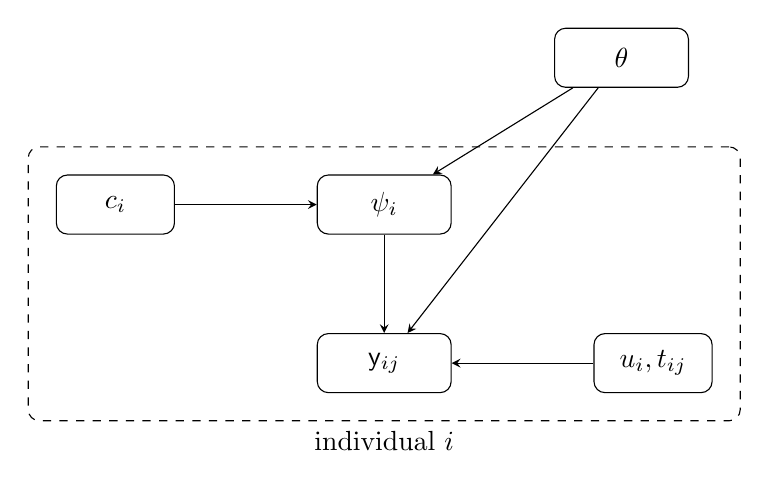
\begin{tikzpicture}[>=stealth, node distance=2.2cm, every node/.style={align=center}]
  \node[draw, rounded corners, minimum width=1.7cm, minimum height=0.75cm] (theta) {\(\theta\)};
  \node[draw, rounded corners, below left=1.1cm and 1.3cm of theta, minimum width=1.7cm, minimum height=0.75cm] (psi) {\(\rv{\psi}_i\)};
  \node[draw, rounded corners, left=1.8cm of psi, minimum width=1.5cm, minimum height=0.75cm] (cov) {\(c_i\)};
  \node[draw, rounded corners, below=1.25cm of psi, minimum width=1.7cm, minimum height=0.75cm] (y) {\(\rv{y}_{ij}\)};
  \node[draw, rounded corners, right=1.8cm of y, minimum width=1.5cm, minimum height=0.75cm] (des) {\(u_i,t_{ij}\)};
  \draw[->] (theta) -- (psi);
  \draw[->] (cov) -- (psi);
  \draw[->] (psi) -- (y);
  \draw[->] (des) -- (y);
  \draw[->] (theta) -- (y);
  \node[draw, dashed, rounded corners, fit=(psi)(y)(cov)(des), inner sep=0.35cm, label=below:{individual \(i\)}] {};
\end{tikzpicture}
\captionof{figure}{A Population PK graphical model. Conditional on \(\theta\), individuals are independent; within an individual, observations depend on the latent individual parameter and the design.}
\end{center}

\subsection{Factorization}

For \(N\) individuals, the joint distribution factorizes as
\[
  p_\theta(y_{1:N},\psi_{1:N}\given c_{1:N},u_{1:N})
  =
  \prod_{i=1}^N
  p_\theta(\psi_i\given c_i)
  p_\theta(y_i\given \psi_i,u_i).
\]
这个 factorization 是 Population PK 所有计算的地基。

Observed data likelihood 是把 latent individual parameters 积掉：
\[
  \lik(\theta;y)
  =
  p_\theta(y_{1:N}\given c_{1:N},u_{1:N})
  =
  \prod_{i=1}^N
  \int
  p_\theta(y_i\given \psi_i,u_i)
  p_\theta(\psi_i\given c_i)
  \dd\psi_i.
\]

\begin{remark}
  这条积分就是 NONMEM、Monolix、SAEM、Laplace、FOCE、importance sampling、MCMC 都绕不开的核心。软件不同，本质都是在处理这个 marginalization。
\end{remark}

\section{What is being estimated?}

\subsection{Population parameters}

Population-level unknowns 可以写成
\[
  \theta=(\mu,B,\Omega,\xi),
\]
其中 \(\mu\) 是 typical fixed effects，\(B\) 是 covariate effects，\(\Omega\) 是 inter-individual variability matrix，\(\xi\) 是 residual error parameters。

Frequentist/maximum-likelihood population modeling asks:
\[
  \widehat\theta_{\pklab{ML}}
  =
  \argmax_\theta \log p_\theta(y).
\]
Full Bayesian modeling asks:
\[
  p(\theta,\psi_{1:N}\given y)
  \propto
  p(\theta)
  \prod_{i=1}^N
  p_\theta(\psi_i\given c_i)
  p_\theta(y_i\given \psi_i,u_i).
\]

\subsection{Individual parameters}

Once \(\widehat\theta\) is estimated, individual parameters are inferred through
\[
  p_{\widehat\theta}(\psi_i\given y_i)
  \propto
  p_{\widehat\theta}(y_i\given \psi_i)
  p_{\widehat\theta}(\psi_i\given c_i).
\]
This is empirical Bayes: the prior-like population distribution is learned from the data, then plugged in.

\begin{center}
\begin{tabularx}{0.96\textwidth}{p{0.22\textwidth}X}
\toprule
Quantity & Meaning \\
\midrule
\(\widehat\theta\) & Estimated population-level model: typical values, variability, covariate effects, residual error. \\
\(\widehat\psi_i^{\pklab{MAP}}\) & Conditional mode for individual \(i\), often called an EBE. \\
\(p(\psi_i\given y_i,\widehat\theta)\) & Full conditional uncertainty for individual \(i\) after seeing his/her data. \\
\(p(\tilde y_i\given y_i,\widehat\theta)\) & Predictive distribution for future observations or dosing scenarios. \\
\bottomrule
\end{tabularx}
\end{center}

\section{The incomplete-data problem}

\subsection{Complete data would be easy}

If we observed both \(y_i\) and \(\psi_i\), estimation of \(\theta\) would be easier because we could maximize
\[
  \log p_\theta(y,\psi)
  =
  \sum_{i=1}^N
  \left[
    \log p_\theta(y_i\given \psi_i)
    +
    \log p_\theta(\psi_i\given c_i)
  \right].
\]
For Gaussian random effects, the second term has familiar sufficient statistics:
\[
  \sum_i h(\psi_i), \qquad
  \sum_i h(\psi_i)h(\psi_i)^T.
\]
But \(\psi_i\) is not observed. We only observe \(y_i\). Therefore Population PK is an incomplete-data model.

\subsection{EM in one line}

6.437 presents EM as a way to maximize observed likelihood by repeatedly replacing missing complete data with its conditional distribution under the current parameter.

Define
\[
  Q(\theta\given \theta^{(k)})
  =
  \E_{\theta^{(k)}}
  \left[
    \log p_\theta(\rv{y},\rv{\psi})
    \given \rv{y}=y
  \right].
\]
Then EM alternates:
\[
  \text{E-step: compute } Q(\theta\given\theta^{(k)}),
\]
\[
  \text{M-step: } \theta^{(k+1)}=\argmax_\theta Q(\theta\given\theta^{(k)}).
\]
In simple exponential-family models this can be analytic. In nonlinear mixed effects models, the conditional distribution \(p_{\theta^{(k)}}(\psi_i\given y_i)\) is rarely analytic.

\section{SAEM: Lavielle's computational bridge}

\subsection{Why stochastic approximation}

SAEM, associated with Lavielle's school and implemented in Monolix, modifies EM for hard incomplete-data problems \cite{kuhn2005saem,lavielle2015mixed}. Instead of exactly computing
\[
  \E_{\theta^{(k)}}[S(\rv{\psi})\given y],
\]
it simulates \(\psi^{(k)}\) from the conditional distribution and updates sufficient statistics through stochastic approximation:
\[
  S_k
  =
  S_{k-1}
  +
  \gamma_k\{S(\psi^{(k)})-S_{k-1}\}.
\]
Then it maximizes the approximate complete-data log-likelihood.

\subsection{The Bayesian heart inside ML}

This is a beautiful point: SAEM is used to find a maximum likelihood estimate of \(\theta\), but each iteration requires sampling from something Bayesian-looking:
\[
  p_{\theta^{(k)}}(\psi_i\given y_i).
\]
So the algorithm lives between worlds:

\begin{itemize}[leftmargin=2em]
  \item population parameter estimation is ML;
  \item individual latent variable update is posterior simulation;
  \item model evaluation uses predictive distributions.
\end{itemize}

This is why learning Bayesian inference first makes Population PK feel much less mysterious.

\subsection{SAEM versus exact EM}

Exact EM can be imagined as:
\begin{quote}
  Replace missing parameters by their exact conditional expectations.
\end{quote}
SAEM is:
\begin{quote}
  Simulate plausible missing parameters and average them carefully over iterations.
\end{quote}
Monte Carlo gives access to complex nonlinear posteriors; stochastic approximation controls noise across iterations.

\section{NONMEM in the same language}

\subsection{Theta, eta, epsilon}

Classical NONMEM notation is usually:
\[
  \begin{aligned}
    \theta &\quad \text{fixed effects},\\
    \eta_i &\sim \Normal(0,\Omega)
      \quad \text{inter-individual random effects},\\
    \epsilon_{ij} &\sim \Normal(0,\Sigma)
      \quad \text{residual errors}.
  \end{aligned}
\]
A typical model:
\[
  \pksym{CL}_i = \theta_{\pklab{CL}}\exp(\eta_{\pklab{CL},i}),
  \qquad
  V_i = \theta_V\exp(\eta_{V,i}),
\]
\[
  y_{ij}
  =
  f(t_{ij};\pksym{CL}_i,V_i,k_{a,i})
  +
  \epsilon_{ij}.
\]
This is exactly the same hierarchy, written through random effects instead of directly through \(p(\psi_i\given c_i;\theta)\).

\subsection{The objective function}

NONMEM's objective function is tied to the marginal likelihood:
\[
  -2\log p_\theta(y)
  =
  -2\sum_i
  \log
  \int
  p_\theta(y_i\given \eta_i)
  p(\eta_i)\,\dd\eta_i.
\]
The hard part is still the integral over \(\eta_i\). Historically, NONMEM made this practical through approximations such as first-order methods and FOCE; later versions also include more simulation-based methods. The algorithmic vocabulary differs, but the inferential object is the same \cite{beal1980nonmem,lindstrom1990nlme}.

\subsection{FO, FOCE, Laplace as approximations}

For intuition:
\begin{itemize}[leftmargin=2em]
  \item \textbf{FO} linearizes the nonlinear model around \(\eta_i=0\). It is fast but can be crude when nonlinearity or variability is large.
  \item \textbf{FOCE} linearizes around each individual's conditional estimate \(\widehat\eta_i\). This respects individual information better.
  \item \textbf{Laplace} approximates the individual integral near the conditional mode, using local curvature.
  \item \textbf{SAEM} uses simulation and stochastic approximation rather than only local linearization.
\end{itemize}

\begin{remark}
  My translation: NONMEM classical methods are local approximations to the same Bayesian-looking integral; SAEM is a stochastic route through the same landscape.
\end{remark}

\section{Full Bayesian Population PK}

\subsection{Adding a prior on population parameters}

Empirical Bayes PopPK estimates \(\theta\), then conditions on \(\widehat\theta\). Full Bayesian PopPK gives \(\theta\) its own prior:
\[
  p(\theta,\psi_{1:N}\given y)
  \propto
  p(\theta)
  \prod_i
  p_\theta(\psi_i\given c_i)
  p_\theta(y_i\given \psi_i,u_i).
\]
Then posterior uncertainty in \(\theta\) is propagated into individual parameters and predictions:
\[
  p(\tilde y\given y)
  =
  \int
  p(\tilde y\given \psi,\theta)
  p(\psi,\theta\given y)
  \dd\psi\,\dd\theta.
\]

\subsection{What changes conceptually}

\begin{center}
\begin{tabularx}{0.96\textwidth}{p{0.24\textwidth}X}
\toprule
Approach & What uncertainty is retained? \\
\midrule
Population ML & \(\widehat\theta\) is a point estimate; uncertainty can be approximated by Fisher information, bootstrap, profile likelihood. \\
Empirical Bayes individual estimation & \(\psi_i\) is inferred conditionally on \(\widehat\theta\); population uncertainty is often ignored in the individual posterior. \\
Full Bayesian & \(\theta\) and \(\psi_i\) are jointly uncertain; posterior and posterior predictive intervals naturally include both levels. \\
\bottomrule
\end{tabularx}
\end{center}

Full Bayesian is not automatically better. It asks for priors, computation, convergence diagnostics, and careful posterior checking. But conceptually it is the cleanest expression of the hierarchy.

\subsection{Bayesian but not mystical}

The useful Bayesian move is not ``believe harder.'' It is:
\[
  \text{state all uncertainty explicitly, then condition on data}.
\]
Population PK already does this for individual parameters. Full Bayesian simply extends the same discipline to population parameters.

\section{Warfarin as a running example}

\subsection{Immediate response fails}

Lavielle's warfarin example is a good teaching case because immediate response is tempting but wrong. Suppose concentration \(C(t)\) is predicted by a PK model and effect is
\[
  E(t)
  =
  1-
  \frac{I_{\max}C(t)}{\pksym{IC}_{50}+C(t)}.
\]
An immediate response model sets
\[
  R(t)=S_0E(t).
\]
If observed PCA reaches its maximum delay long after peak concentration, the concentration-effect scatter shows hysteresis. Then \(C(t)\to R(t)\) is not instantaneous.

\subsection{Effect compartment}

One repair is to introduce a latent effect-site concentration:
\[
  \frac{\dd C_e(t)}{\dd t}
  =
  k_{e0}\{C(t)-C_e(t)\}.
\]
Then effect depends on \(C_e(t)\), not directly on \(C(t)\):
\[
  E_e(t)
  =
  1-
  \frac{I_{\max}C_e(t)}{\pksym{IC}_{50}+C_e(t)}.
\]
This is a perfect example of Bayesian modeling logic: when data show systematic structure not explained by current latent variables, introduce a better latent state.

\subsection{Indirect response}

Warfarin also has a biological mechanism: inhibition of prothrombin synthesis. An indirect response model can write
\[
  \frac{\dd R(t)}{\dd t}
  =
  k_{\mathrm{in}}
  \left(
    1-\frac{I_{\max}C(t)}{\pksym{IC}_{50}+C(t)}
  \right)
  -
  k_{\mathrm{out}}R(t).
\]
This model no longer says drug directly changes measured response. It says drug changes the production process; the measured response follows through turnover. That is more mechanistic and often more interpretable.

\section{Model evaluation as posterior criticism}

\subsection{Prediction before p-values}

Lavielle emphasizes model diagnostics and visual predictive checks. In Bayesian language, this is posterior predictive criticism:
\[
  \tilde y \sim p(\tilde y\given y),
\]
then compare simulated \(\tilde y\) with observed \(y\).

VPC asks: if my model were the data-generating mechanism, would data like mine look ordinary? If not, where does it fail: absorption phase, terminal phase, variability, covariate groups, below quantification limit, dropout?

\subsection{Residuals need context}

Common residuals such as IWRES, CWRES, NPDE are not just software outputs. They are attempts to transform model misfit into a scale where remaining noise should look simple. If residuals still show time trend, concentration dependence, covariate dependence, or heavy tails, the probability model is misspecified.

\subsection{Model selection}

6.437's ``modeling as inference'' view is helpful: a model is an approximation to the true data distribution. Selection should not be reduced to one number.

\begin{itemize}[leftmargin=2em]
  \item Likelihood/AIC/BIC answer an approximation-complexity tradeoff.
  \item Likelihood ratio tests compare nested models under regularity assumptions.
  \item VPC/PPC ask whether predictive behavior is credible.
  \item Clinical utility asks whether the model is good enough for the decision.
\end{itemize}

\begin{remark}
  The most PopPK-specific danger is choosing a model because OFV improves while ignoring whether the resulting random effects, shrinkage, covariate effects, and predictions make pharmacological sense.
\end{remark}

\section{How to read a PopPK paper}

\subsection{The inference checklist}

When I read a Population PK paper, I want to reconstruct the graphical model:

\begin{enumerate}[leftmargin=2em]
  \item What are the observations \(\rv{y}_{ij}\)? Concentration only, PK/PD joint, categorical, time-to-event?
  \item What is the structural model \(f(t;\psi_i,u_i)\)?
  \item Which parameters are individual-specific \(\psi_i\), and which are population-level \(\theta\)?
  \item What transformations ensure parameter constraints? log for positive, logit for fractions?
  \item What covariates enter \(h(\psi_i)\)?
  \item What residual error model defines \(p(y_i\given\psi_i)\)?
  \item What algorithm approximates the likelihood or posterior?
  \item How are individual estimates summarized, and is shrinkage reported?
  \item What diagnostics check predictive adequacy?
  \item What decision does the model support?
\end{enumerate}

\subsection{Reading NONMEM output}

A NONMEM run can be read as a probabilistic story:

\begin{itemize}[leftmargin=2em]
  \item \(\theta\): learned typical physiology and covariate effects.
  \item \(\Omega\): learned unexplained between-subject variability.
  \item \(\Sigma\): learned observation noise.
  \item \(\eta_i\): posterior-ish individual deviation from the typical subject.
  \item OFV: approximation to marginal log-likelihood.
  \item CWRES/IWRES: checks on conditional observation model.
  \item VPC: check on population predictive distribution.
\end{itemize}

Once read this way, NONMEM stops being an opaque command-line tradition and becomes an inference engine with a particular notation and approximation culture.

\section{Slow source map}

\subsection{What this expansion is trying to do}

The first draft gave the right high-level bridge but it moved too quickly.  A reader who has not taken 6.008 or 6.437 needs more than a dictionary between symbols.  They need to feel why the symbols were invented.  They need to see how a small probability question becomes a dosing question, how a latent-variable question becomes a mixed-effects model, and how a computational question becomes NONMEM, SAEM, or MCMC.

The expanded version therefore follows a slower route:
\[
  \text{probability object}
  \longrightarrow
  \text{conditioning}
  \longrightarrow
  \text{decision}
  \longrightarrow
  \text{hierarchy}
  \longrightarrow
  \text{algorithm}
  \longrightarrow
  \text{pharmacological judgment}.
\]
The order matters.  If we begin with NONMEM syntax, the reader sees THETA, ETA, EPSILON, OMEGA, and SIGMA as a software dialect.  If we begin with Lavielle's joint distribution but skip inference, the reader sees a clean model and does not know what is hard about it.  If we begin with Bayes rule but skip PK, the reader understands updating but not why individual parameters are biologically meaningful.  The point of this note is to keep all three views alive at the same time.

\begin{remark}
  I will use ``Bayesian'' in two levels.  In the strict level, a Bayesian model puts priors on all unknown quantities, including population parameters.  In the broader inferential level, a PopPK model is already Bayesian in spirit because individual parameters are latent variables updated by individual observations under a population distribution.  Much of classical Population PK is maximum likelihood for \(\theta\), but conditional inference for \(\psi_i\).  That mixed posture is not a defect; it is exactly why the field is intellectually interesting.
\end{remark}

\subsection{The three texts in one sentence each}

The 6.008 notes teach the grammar of probability modeling: decide what the sample space is, assign a probability law, condition on observations, and compute probabilities, expectations, decisions, or approximations \cite{mit6008notes}.  The 6.437 notes deepen the grammar: inference is decision-making under loss, likelihood ratios compare hypotheses, posterior distributions summarize unknown quantities, information measures compare probability laws, EM and MCMC appear when exact marginalization is hard, and asymptotic arguments explain what happens when data are abundant \cite{mit6437notes}.  Lavielle's book gives the pharmacometric stage on which the grammar acts: observations \(y_i\), individual parameters \(\psi_i\), population parameters \(\theta\), covariates \(c_i\), designs \(u_i\), tasks, methods, and tools \cite{lavielle2015mixed}.

I want the reader to learn a habit:
\[
  \text{When a PopPK paper writes a model, redraw the probability law.}
\]
The redraw should answer four questions:
\begin{enumerate}[leftmargin=2em]
  \item What is observed?
  \item What is latent?
  \item What is fixed by design?
  \item What is being inferred or decided?
\end{enumerate}
Only after these four questions are stable should we ask which software or algorithm is being used.

\subsection{A source hierarchy rather than a literature review}

This is not a literature review.  A literature review would place many papers side by side and compare claims.  Here I am building a reading hierarchy.  The hierarchy is:
\[
  \begin{array}{lll}
  \text{6.008} & \text{asks} & \text{What probability model are we even talking about?}\\
  \text{6.437} & \text{asks} & \text{What inference, decision, or approximation follows from that model?}\\
  \text{Lavielle} & \text{asks} & \text{How is this hierarchy represented, estimated, diagnosed, and used?}\\
  \textit{NONMEM} & \text{asks} & \text{How does this object appear in a historical pharmacometric syntax?}
  \end{array}
\]
When the four rows disagree, the note slows down.  For example, an EBE in NONMEM syntax may look like a subject's true clearance.  But from the 6.437 view it is a posterior summary under a loss function or approximation.  From Lavielle's view it is the estimation of an individual parameter conditional on an estimated population model.  From 6.008's view it is a random variable transformed after conditioning.  These are not pedantic distinctions.  They decide whether we can interpret a covariate effect, trust a dose adjustment, or compare two models.

\section{6.008 carefully: probability law before Bayes rule}

\subsection{The sample point is not a blood concentration}

The first subtle point is that a sample point is not necessarily a single blood concentration.  If a subject receives a dose regimen and produces a longitudinal record, a natural sample outcome contains the entire observed trajectory:
\[
  y_i=(y_{i1},\ldots,y_{in_i}).
\]
If the model includes unobserved biology, the outcome may be enlarged to
\[
  (y_i,\psi_i),
\]
where \(\psi_i\) might contain clearance, volume, absorption rate, baseline response, turnover parameters, or sensitivity parameters.  If the design itself is randomized, the outcome may also include \(u_i\).  If dropout is informative, the event time of dropout must become part of the outcome.  The modeler is already making a scientific claim when deciding what belongs in the sample space.

This is the first place where Population PK becomes more subtle than curve fitting.  Curve fitting says: here are points and here is a curve.  Probability modeling says: here is a law that could have generated the record, the latent physiology, the measurement noise, and possibly the sampling schedule.  A curve is only one conditional mean or median inside that law.

\begin{eg}
  Suppose two subjects have the same observed concentration at two early time points.  One model treats this as evidence that their clearances are similar.  Another model says the sampling schedule is too early to distinguish clearance from volume.  The observed numbers are the same, but the sample space and latent structure create different inferential meanings.
\end{eg}

\subsection{Events are clinical subsets}

In 6.008, an event is a subset of the sample space.  In PopPK, this sounds abstract until we write clinical events:
\[
  A_1=\{\tilde C_{\min}<C_{\mathrm{eff}}\},
  \qquad
  A_2=\{\tilde C_{\max}>C_{\mathrm{tox}}\},
  \qquad
  A_3=\{\textit{AUC}_{0,\tau}\in[L,U]\}.
\]
These are not decorative.  They are what dosing decisions are often about.  A model that estimates \(\textit{CL}_i\) well but cannot answer \(P(A_2\mid y_i)\) may be less useful than a model with slightly rougher parameter estimates but better predictive calibration in the clinically relevant tail.

This is why the 6.008 language should come before software.  If the event has not been named, the analysis cannot know what probability matters.  The event may be exposure-based, response-based, toxicity-based, adherence-based, or survival-based.  Each event changes the target of inference.

\subsection{Probability laws as commitments}

A probability law is a commitment about variation.  In a simple one-compartment model, one might write
\[
  y_{ij}=f(t_{ij};\textit{CL}_i,V_i,u_i)+\varepsilon_{ij},
  \qquad
  \varepsilon_{ij}\sim\Normal(0,\sigma^2).
\]
This commits to additive Gaussian residual error on the concentration scale.  If instead we write
\[
  \log y_{ij}=\log f(t_{ij};\textit{CL}_i,V_i,u_i)+\varepsilon_{ij},
  \qquad
  \varepsilon_{ij}\sim\Normal(0,\sigma^2),
\]
we commit to approximately lognormal multiplicative error.  The structural curve may be the same, but the probability law is not the same.  Low concentrations, high concentrations, BLQ observations, and extreme residuals will be treated differently.

Lavielle's emphasis on description, representation, and implementation is useful here.  The description may say ``proportional residual error.''  The mathematical representation might be a lognormal observation density.  The implementation might be NONMEM code, Mlxtran code, Stan code, or an R function.  A reader should be able to move between these without changing the underlying probability law.

\subsection{The law of total probability is the population idea}

The law of total probability is the first real bridge to Population PK.  For a new observation \(y_i\),
\[
  p_\theta(y_i\mid c_i,u_i)
  =
  \int p_\theta(y_i\mid \psi_i,u_i)
       p_\theta(\psi_i\mid c_i)\,\dd \psi_i.
\]
This is not a technical afterthought.  It is the population approach in one line.  The individual parameter \(\psi_i\) is not observed, so the likelihood of the observed record averages over plausible individual physiologies.  The averaging is weighted by the population distribution.  That is what allows sparse individual data to borrow strength from the group.

The same identity also explains why nonlinear mixed-effects estimation is hard.  The integrand contains a nonlinear forward model, possibly an ODE solution, and a high-dimensional random effect.  The integral is rarely closed-form.  Therefore algorithms enter not because pharmacometricians enjoy algorithms, but because the probability law demands marginalization.

\subsection{Bayes rule as individual reweighting}

For an individual subject, Bayes rule gives
\[
  p_\theta(\psi_i\mid y_i,c_i,u_i)
  =
  \frac{
    p_\theta(y_i\mid \psi_i,u_i)p_\theta(\psi_i\mid c_i)
  }{
    \int p_\theta(y_i\mid \psi_i,u_i)p_\theta(\psi_i\mid c_i)\,\dd\psi_i
  }.
\]
The numerator has two forces.  The population distribution says which physiologies are plausible before seeing the subject's data.  The individual likelihood says which physiologies explain the observed concentrations or responses.  The denominator normalizes the result and is also the individual marginal likelihood contribution.

This equation is the cleanest way to understand shrinkage.  If \(y_i\) is rich, the likelihood is sharp and the posterior moves toward the individual evidence.  If \(y_i\) is sparse or noisy, the likelihood is broad and the posterior remains closer to the population distribution.  Shrinkage is not a software artifact.  It is the geometry of conditional probability under limited information.

\section{Random variables as pharmacological summaries}

\subsection{A random variable is a question asked of the outcome}

6.008 treats a random variable as a function from outcomes to numbers.  In PopPK, that function is often a pharmacological summary:
\[
  \textit{AUC}_i=\frac{D_i}{\textit{CL}_i},
  \qquad
  t_{1/2,i}=\frac{\log 2}{k_i},
  \qquad
  C_{\max,i}=\max_t C_i(t).
\]
Once \(\textit{CL}_i\), \(k_i\), or the whole curve \(C_i(t)\) is uncertain, these summaries are uncertain too.  The habit is therefore:
\[
  \text{do not only report a transformed point estimate; transform the uncertainty.}
\]
The posterior distribution of \(\textit{CL}_i\) induces a posterior distribution of \(\textit{AUC}_i\).  The posterior predictive distribution of future concentrations induces probabilities of clinical target attainment.  This is where the random-variable language becomes directly useful.

\subsection{Expectations are summaries, not reality}

An expectation is often useful:
\[
  \E(\textit{AUC}_i\mid y_i)
  =
  \int \frac{D_i}{\textit{CL}_i}p(\textit{CL}_i\mid y_i)\,\dd \textit{CL}_i.
\]
But the expectation is not the same as the whole posterior distribution.  In asymmetric or safety-critical problems, the upper tail may matter more than the mean.  A dosing rule based on \(\E(\textit{AUC}_i\mid y_i)\) may be inferior to a rule based on
\[
  P(\textit{AUC}_i>U\mid y_i)
\]
if toxicity risk is the central concern.  This is where 6.008 expectation leads naturally into 6.437 decision theory.

\subsection{Independence is a modeling assumption}

It is common to write
\[
  y_{ij}\indep y_{ik}\mid \psi_i,\theta
\]
for two observations from the same subject.  This does not mean the observations are marginally independent.  They are connected through the same latent individual parameter \(\psi_i\).  Conditional independence is a statement about what remains after we condition on the relevant latent structure.

This distinction is crucial for repeated measures.  If a model treats observations as independent without individual random effects, it may underestimate uncertainty because it ignores within-subject correlation.  If a model includes \(\psi_i\), much of the dependence is explained by shared physiology.  Remaining residual dependence may still exist through assay drift, disease dynamics, adherence, or unmodeled feedback.  A good PopPK reader always asks: independent after conditioning on what?

\section{Decision theory before dosing software}

\subsection{Estimation is a decision with a loss}

6.437 makes explicit what is implicit in many reports: an estimate is a decision.  If we report a posterior mean, we are usually acting as if squared-error loss is relevant.  If we report a posterior median, absolute-error loss is often lurking.  If we report a MAP or EBE mode, a zero-one or local mode-seeking logic is being used.  These summaries can differ when the posterior is skewed or multimodal.

For individual dosing, the decision may not be an estimate at all.  The action is a dose \(a\), and the loss might penalize underexposure and overexposure differently:
\[
  L(a,\tilde y)
  =
  \lambda_{\mathrm{low}}1\{\tilde C_{\min}(a)<C_{\mathrm{eff}}\}
  +
  \lambda_{\mathrm{high}}1\{\tilde C_{\max}(a)>C_{\mathrm{tox}}\}.
\]
The Bayesian action minimizes posterior predictive risk:
\[
  a^\star
  =
  \argmin_a \E\{L(a,\tilde{\rv y})\mid y_i\}.
\]
This formula is more honest than saying ``choose the dose that hits the target concentration.''  It forces the modeler to say what failure means.

\subsection{Why clinical asymmetry matters}

In some drugs, underdosing is the main danger.  In others, toxicity dominates.  For warfarin, both sides matter: too little anticoagulation fails to prevent thrombosis; too much increases bleeding risk.  A symmetric statistical error metric may not match this clinical asymmetry.  The 6.437 move is to put the asymmetry into the loss.

The loss does not need to be final or perfectly quantified.  Even a qualitative loss table is clarifying:
\[
  \begin{array}{c|cc}
  & \text{true exposure low} & \text{true exposure high}\\ \hline
  \text{increase dose} & \text{benefit} & \text{toxicity risk}\\
  \text{decrease dose} & \text{failure risk} & \text{benefit}
  \end{array}
\]
Once written, we can ask whether the PopPK model actually provides the predictive quantities needed to evaluate the table.

\subsection{The danger of decision-blind model selection}

Model selection is often performed with OFV, AIC, BIC, diagnostic plots, and VPC.  These are valuable, but they do not automatically answer the decision question.  A model may improve OFV by fitting a minor absorption feature while leaving dose-relevant trough prediction unchanged.  Another model may have similar OFV but better tail calibration for a high-risk subgroup.

The decision-theoretic reading is:
\[
  \text{Model adequacy is relative to the downstream action.}
\]
This does not excuse sloppy modeling.  It prevents a narrow criterion from masquerading as clinical adequacy.

\section{Graphical models for the population approach}

\subsection{The basic plate}

A minimal population PK graphical model can be written as
\[
  \theta \longrightarrow \psi_i \longrightarrow y_i,
  \qquad
  c_i \longrightarrow \psi_i,
  \qquad
  u_i \longrightarrow y_i,
  \qquad
  i=1,\ldots,N.
\]
Here \(\theta\) contains population-level parameters, \(c_i\) covariates, \(u_i\) the design or dosing regimen, \(\psi_i\) individual parameters, and \(y_i\) observations.  The factorization is
\[
  p_\theta(y_{1:N},\psi_{1:N}\mid c_{1:N},u_{1:N})
  =
  \prod_{i=1}^N
  p_\theta(\psi_i\mid c_i)
  p_\theta(y_i\mid \psi_i,u_i).
\]
This is the mathematical reason the subject-level records can be conditionally independent given the population model and covariates.  It is also the reason likelihood computation separates into individual integrals:
\[
  p_\theta(y_{1:N}\mid c_{1:N},u_{1:N})
  =
  \prod_{i=1}^N
  \int
  p_\theta(\psi_i\mid c_i)
  p_\theta(y_i\mid \psi_i,u_i)
  \,\dd\psi_i.
\]

\subsection{What the plate hides}

The plate is compact, but it hides important choices.  Does \(u_i\) include only planned dose and sampling times, or also adherence?  Are covariates \(c_i\) fixed, measured with error, or time-varying?  Is dropout independent given \(\psi_i\), or does worsening disease affect both dropout and response?  Does disease progression introduce another latent state?  Does the residual error have serial correlation?

Each of these choices changes the graph.  For instance, if dropout time \(T_i\) is informative, the observation model might become
\[
  p(y_i,T_i\mid \psi_i,u_i)
  =
  p(y_i\mid T_i,\psi_i,u_i)p(T_i\mid \psi_i,u_i),
\]
or a joint latent disease model might be needed.  Ignoring this can bias estimation because the observed record is no longer a simple random slice of the intended process.

\subsection{The graph as a reading tool}

When reading a paper, redraw the graph before judging the model.  If the paper says ``renal function was a significant covariate on clearance,'' draw \(c_i\to \textit{CL}_i\).  If the paper says ``inter-occasion variability was included on bioavailability,'' draw an occasion-level random effect below the subject-level random effect.  If the paper says ``BLQ data were handled with M3,'' draw the censoring event as part of the observation mechanism.

This is not busywork.  It reveals whether a claim is about the structural model, the residual model, the covariate model, the sampling process, or the decision rule.

\section{Lavielle's joint-distribution thesis}

\subsection{A model is not only a structural equation}

One of Lavielle's most useful claims is that a model is a joint probability distribution.  A structural equation is only one component.  In continuous PK data, the full model needs at least:
\[
  p_\theta(y_i,\psi_i\mid c_i,u_i)
  =
  p_\theta(y_i\mid \psi_i,u_i)
  p_\theta(\psi_i\mid c_i).
\]
If \(\theta\) is also random, a Bayesian extension adds \(p(\theta)\).  If covariates or dosing records are modeled as random, they also enter.  But even the basic two-layer expression already changes how we think.  The question is not merely whether \(f(t;\psi_i)\) fits the observed curve.  The question is whether the joint law explains individual profiles, between-subject variability, residual noise, and prediction targets.

\subsection{Description, representation, implementation}

Lavielle's separation of description, representation, and implementation is a powerful anti-confusion device.

\begin{itemize}[leftmargin=2em]
  \item The \term{description} is the scientific story: clearance varies between individuals; body weight may explain part of that variation; concentration is measured with assay noise.
  \item The \term{representation} is the mathematical probability law: \(\textit{CL}_i=\textit{CL}_{\pop}(\textit{WT}_i/70)^\beta\exp(\eta_{\textit{CL},i})\), \(\eta_i\sim\Normal(0,\Omega)\), and an observation density.
  \item The \term{implementation} is the computational form: NONMEM control stream, Mlxtran project, Stan program, Monolix task, or a custom likelihood.
\end{itemize}

Many arguments in modeling are actually category errors between these levels.  Someone may criticize an implementation detail as if it were a scientific description.  Someone else may defend a scientific story without showing a coherent probability law.  A careful PopPK note keeps the levels separate.

\subsection{A complete PopPK law}

For a common continuous-data model, one representation is:
\[
  \eta_i\sim\Normal(0,\Omega),
  \qquad
  h(\psi_i)=h(\psi_{\pop})+B c_i+\eta_i,
\]
\[
  C_{ij}=f(t_{ij};\psi_i,u_i),
  \qquad
  y_{ij}=C_{ij}+g(C_{ij};a,b)\varepsilon_{ij},
  \qquad
  \varepsilon_{ij}\iid\Normal(0,1).
\]
The transformation \(h\) is often logarithmic for positive parameters.  The residual scale \(g\) might be constant, proportional, or combined.  The covariate term \(Bc_i\) may be linear, allometric, categorical, nonlinear, or absent.

This one representation already contains many modeling commitments.  Does every parameter have an \(\eta\)?  Is \(\Omega\) diagonal?  Are residuals independent?  Are covariates centered?  Are parameters constrained by transformation or by truncation?  Each answer changes inference.

\section{Observation models}

\subsection{Continuous observations}

For continuous concentrations or responses, Lavielle's Chapter 4 emphasizes that the observation model is not merely ``add error.''  It defines the conditional density \(p(y_i\mid\psi_i)\).  With independent residuals,
\[
  p(y_i\mid\psi_i)
  =
  \prod_{j=1}^{n_i}
  \frac{1}{g_{ij}\sqrt{2\pi}}
  \exp\left\{
    -\frac{1}{2}
    \left(\frac{y_{ij}-f_{ij}(\psi_i)}{g_{ij}}\right)^2
  \right\}.
\]
Here \(f_{ij}(\psi_i)=f(t_{ij};\psi_i,u_i)\), and \(g_{ij}\) may depend on the prediction.  The residual error model is therefore part of the likelihood geometry.  It determines which deviations are surprising.

For concentration data spanning orders of magnitude, proportional or lognormal error can be more plausible than additive error.  For responses with bounded ranges, transformations or non-Gaussian likelihoods may be needed.  For BLQ data, replacing observations by a fixed value can distort the likelihood; censoring-based likelihood terms are more principled.

\subsection{Count, categorical, and time-to-event observations}

Lavielle's broader point is that the population approach is not limited to continuous PK data.  If \(y_i\) is a count, a Poisson or negative-binomial observation model may be appropriate.  If \(y_i\) is categorical, the structural model may define category probabilities.  If \(y_i\) is a time-to-event outcome, the model may define a hazard or survival function.

The Bayesian inference language is unchanged:
\[
  p_\theta(y_i\mid\psi_i)
\]
is still the conditional observation law.  What changes is the family of densities or probabilities.  This is important for PK/PD because pharmacological effects are often not clean continuous laboratory measurements.  Pain scores, toxicity grades, event times, response categories, and dropout can all be modeled in the same hierarchical grammar.

\subsection{Residuals are derived objects}

Residuals are not raw facts.  They are transformations defined by a fitted model.  An individual weighted residual, a conditional weighted residual, and an NPDE answer different questions.  A residual plot is therefore a diagnostic of a probability law, not simply a scatterplot of errors.

If residuals show time trend, the structural model may be missing dynamics.  If residual variance grows with prediction, the error model may be wrong.  If residuals differ by covariate group, the covariate model may be incomplete.  If residuals have heavy tails, a Gaussian observation density may be fragile.  Diagnostic reading is posterior criticism in practical clothing.

\section{Individual parameter models}

\subsection{The population distribution}

The individual parameter model says how people differ.  A common form is
\[
  \log \textit{CL}_i
  =
  \log \textit{CL}_{\pop}
  +\beta_{\textit{WT}}\log(\textit{WT}_i/70)
  +\eta_{\textit{CL},i},
  \qquad
  \eta_{\textit{CL},i}\sim\Normal(0,\omega_{\textit{CL}}^2).
\]
This is not only a regression.  It is a probability distribution for individual clearance.  The covariate term explains systematic variability; the random effect represents remaining between-subject variability.  The log transform ensures positivity and often makes multiplicative biological variability more plausible.

The model answers two different questions at once:
\[
  \text{What is typical for a covariate profile?}
  \qquad
  \text{How much unexplained variability remains?}
\]
Confusing these questions is common.  A covariate may have a statistically visible effect but leave most variability unexplained.  Conversely, a covariate may explain important variability in a subgroup even if global fit changes modestly.

\subsection{Covariates are not causal by default}

A covariate model is often written as if it explains biology:
\[
  \textit{CL}_i=\textit{CL}_{\pop}(\textit{WT}_i/70)^{\beta}\exp(\eta_i).
\]
But the coefficient \(\beta\) is causal only under additional assumptions about design, confounding, measurement, and biology.  In observational PopPK datasets, covariates can be proxies.  Renal function, age, weight, disease severity, dose history, and comedications may be entangled.

The Bayesian reading is cautious: the covariate model changes \(p(\psi_i\mid c_i)\).  Whether that conditional association supports intervention is a separate causal question.  This distinction matters if the model is used to recommend dose changes based on modifiable covariates.

\subsection{Inter-occasion variability}

Sometimes a subject's parameter changes across occasions:
\[
  \log \textit{CL}_{ik}
  =
  \log \textit{CL}_{\pop}
  +\eta_{i}
  +\kappa_{ik},
\]
where \(\eta_i\) is between-subject variability and \(\kappa_{ik}\) is inter-occasion variability.  This adds another hierarchical layer.  The graph now has subject-level and occasion-level latent variables.

This is not a technical ornament.  Without inter-occasion variability, the model may force within-subject changes into residual error or distort between-subject variability.  With it, the model can distinguish persistent individual differences from occasion-specific fluctuations.

\section{Structural PK as a forward map}

\subsection{The model as a deterministic solver inside probability}

The structural PK model maps parameters and design to predictions:
\[
  f(t;\psi_i,u_i).
\]
For a one-compartment IV bolus model,
\[
  C_i(t)=\frac{D_i}{V_i}\exp\left(-\frac{\textit{CL}_i}{V_i}t\right).
\]
For extravascular dosing with first-order absorption, the formula is more complicated, and for many systems the prediction is obtained by solving ODEs.  But the inferential role is the same: \(f\) is the deterministic forward map inside the stochastic observation law.

This separation is useful.  The PK equation by itself is not a statistical model.  The statistical model begins when we say how \(\psi_i\) varies and how \(y_i\) deviates from \(f\).  The forward map provides pharmacological structure; probability wraps uncertainty around it.

\subsection{Identifiability and design}

Sparse sampling can make parameters hard to distinguish.  In a one-compartment model, early samples may inform volume and absorption; later samples inform elimination; troughs may inform clearance but not absorption.  A model can be algebraically correct and still weakly identified by the design.

This is where \(u_i\) matters.  Doses and sampling times are not administrative details; they determine the likelihood's shape.  Two designs with the same number of samples can produce very different information about \(\psi_i\).  A Bayesian posterior under a weak design will remain broad or shrink strongly toward the population distribution.

\subsection{PK/PD coupling}

PK/PD modeling introduces another forward layer:
\[
  \psi_i^{\textit{PK}}\longrightarrow C_i(t),
  \qquad
  \psi_i^{\textit{PD}}\longrightarrow R_i(t),
  \qquad
  C_i(t)\longrightarrow R_i(t).
\]
Immediate effect models, effect-compartment models, and indirect response models differ in how concentration drives response.  The difference is not cosmetic.  It represents different biological stories about delay, turnover, and mechanism.

Warfarin is a useful example because concentration and response are not synchronized.  A direct immediate response model can fit poorly because the pharmacodynamic effect is delayed relative to concentration.  Introducing an effect compartment or turnover model changes the latent state, the forward map, and the interpretation of parameters.

\section{Marginal likelihood and the hard integral}

\subsection{The individual contribution}

The population likelihood is built from individual contributions:
\[
  L(\theta)
  =
  \prod_{i=1}^{N}
  \ell_i(\theta),
  \qquad
  \ell_i(\theta)
  =
  \int
  p_\theta(y_i\mid\psi_i)
  p_\theta(\psi_i\mid c_i)
  \,\dd\psi_i.
\]
The integral is the mathematical center of classical PopPK.  It is also the bridge between Bayesian and frequentist language.  The integrand contains a prior-like population distribution and an individual likelihood.  The maximum likelihood estimate chooses \(\theta\) so the observed records have high marginal probability.

This is why individual posteriors appear even in an ML workflow.  During computation or post hoc estimation, we often need
\[
  p_{\widehat\theta}(\psi_i\mid y_i,c_i)
  \propto
  p_{\widehat\theta}(y_i\mid \psi_i)
  p_{\widehat\theta}(\psi_i\mid c_i).
\]
The population parameters are estimated by ML, but the individual parameters are interpreted through conditional distributions.

\subsection{Why approximation enters}

If \(f\) is nonlinear and \(\psi_i\) is multidimensional, \(\ell_i(\theta)\) is hard.  Several approximation cultures arise:
\begin{itemize}[leftmargin=2em]
  \item Linearize the model and approximate the integral locally.
  \item Use Laplace approximation around an individual mode.
  \item Use Gaussian quadrature when dimension permits.
  \item Use Monte Carlo or importance sampling.
  \item Use EM or SAEM by treating \(\psi_i\) as missing data.
\end{itemize}
These are not competing philosophies so much as different responses to the same integral.

\subsection{The individual mode is not the integral}

The conditional mode
\[
  \widehat\psi_i
  =
  \argmax_{\psi_i}
  p_{\widehat\theta}(y_i\mid\psi_i)p_{\widehat\theta}(\psi_i\mid c_i)
\]
is useful, but it is not the same as marginalization.  Replacing an integral by a mode can be accurate in some local Gaussian settings and poor in skewed, weakly informed, or multimodal settings.  This is one reason FOCE, Laplace, SAEM, and MCMC can disagree in difficult models.

\section{EM, SAEM, and missing individual parameters}

\subsection{Complete data}

If \(\psi_i\) were observed, the complete-data log-likelihood would be
\[
  \log p_\theta(y_{1:N},\psi_{1:N})
  =
  \sum_{i=1}^{N}
  \log p_\theta(y_i\mid\psi_i)
  +
  \sum_{i=1}^{N}
  \log p_\theta(\psi_i\mid c_i).
\]
This is easier than the observed likelihood because the integral disappears.  EM uses this easier object by averaging it under the current conditional distribution of missing data.

\subsection{The EM idea}

At iteration \(k\), EM constructs
\[
  Q(\theta\mid\theta^{(k)})
  =
  \E_{\theta^{(k)}}\{
    \log p_\theta(y,\psi)
    \mid y
  \}.
\]
Then it chooses a new \(\theta\) that improves or maximizes \(Q\).  The 6.437 view is that EM is a lower-bound or alternating-optimization method.  The PopPK view is that EM repeatedly imputes the latent individual parameters probabilistically and then refits the population model.

\subsection{SAEM's pharmacometric value}

In nonlinear mixed-effects models, the expectation in \(Q\) may be hard.  SAEM replaces exact expectation with stochastic approximation.  It simulates plausible individual parameters from conditional distributions, updates sufficient statistics gradually, and then maximizes an approximate complete-data criterion.

This gives a very useful conceptual summary:
\[
  \text{SAEM is ML for population parameters using Bayesian-looking draws for individuals.}
\]
The algorithm is not fully Bayesian unless \(\theta\) also receives a prior and is sampled or integrated.  But the conditional simulation step is naturally understood by anyone comfortable with posterior distributions.

\section{NONMEM as a notation and approximation culture}

\subsection{THETA, ETA, EPSILON}

NONMEM's notation can be translated:
\[
  \theta \leftrightarrow \textit{THETA},
  \qquad
  \eta_i \leftrightarrow \textit{ETA},
  \qquad
  \varepsilon_{ij} \leftrightarrow \textit{EPSILON},
\]
\[
  \Omega \leftrightarrow \textit{OMEGA},
  \qquad
  \Sigma \leftrightarrow \textit{SIGMA}.
\]
A line such as
\[
  \textit{CL}_i=\textit{TVCL}\exp(\eta_{\textit{CL},i})
\]
is not just code.  It is a distributional statement:
\[
  \log \textit{CL}_i\sim\Normal(\log \textit{TVCL},\omega_{\textit{CL}}^2).
\]
This translation makes NONMEM less mysterious.  It is a compact language for hierarchical probability models.

\subsection{FO, FOCE, Laplace}

First-order methods approximate the nonlinear model around typical random effects.  FOCE improves this by expanding around individual conditional estimates.  Laplace uses curvature near the conditional mode to approximate the integral.  These methods are local.  They can be efficient and powerful, but the reader should know what is being approximated.

The target remains the marginal likelihood:
\[
  \int p(y_i\mid\eta_i,\theta)p(\eta_i\mid\Omega)\,\dd\eta_i.
\]
The approximations differ in how they replace this hard integral by something tractable.  This makes the comparison with SAEM precise: SAEM uses simulation and stochastic approximation; FOCE/Laplace use local approximation.

\subsection{EBEs and shrinkage}

An empirical Bayes estimate is often a conditional mode or related summary under \(\widehat\theta\).  It is useful for diagnostics and interpretation, but it is not a direct observation.  High shrinkage means individual data are not informative enough to pull estimates far from the population.  Using high-shrinkage EBEs for covariate discovery can be misleading because the apparent individual variability has been compressed by the model.

The Bayesian language prevents overinterpretation:
\[
  \widehat\eta_i
  \quad\text{is a summary of}\quad
  p_{\widehat\theta}(\eta_i\mid y_i),
  \quad\text{not a measured biological truth.}
\]

\section{Model evaluation as calibrated imagination}

\subsection{Posterior predictive thinking}

Model evaluation asks whether data generated from the fitted model resemble the observed data in scientifically relevant ways.  In Bayesian notation, simulate
\[
  \tilde y\sim p(\tilde y\mid y)
\]
or, in an ML PopPK workflow, simulate from the fitted population model
\[
  \tilde\psi_i\sim p_{\widehat\theta}(\psi_i\mid c_i),
  \qquad
  \tilde y_i\sim p_{\widehat\theta}(y_i\mid \tilde\psi_i,u_i).
\]
Then compare observed and simulated summaries.

This is calibrated imagination: the model imagines new datasets.  Diagnostics ask whether those imagined datasets look like the real one.

\subsection{Visual predictive checks}

A VPC is not merely a plot.  It is a comparison between observed summaries and predictive summaries under the model.  The reader should ask:
\begin{enumerate}[leftmargin=2em]
  \item Are simulations using the same design as the observed study?
  \item Are covariate groups respected?
  \item Are BLQ and missing data mechanisms handled consistently?
  \item Are prediction intervals checking the part of the distribution that matters clinically?
  \item Does the VPC hide individual-level failure by pooling too aggressively?
\end{enumerate}
The 6.008/6.437 language clarifies the object: a VPC checks a function of the predictive distribution.

\subsection{Model selection as multiple evidence streams}

No single criterion should dominate.  OFV and likelihood compare fit under a statistical criterion.  AIC and BIC penalize complexity differently.  Bootstrap and Fisher information describe parameter uncertainty.  VPC and PPC examine predictive behavior.  Residual diagnostics examine local misfit.  Clinical decision analysis asks whether the model is adequate for its intended use.

The mature view is not ``choose the lowest number.''  It is:
\[
  \text{Choose the model whose probability law is adequate for the scientific and clinical task.}
\]

\section{Warfarin re-read}

\subsection{Why the example is instructive}

Warfarin is pedagogically rich because the PK and PD time scales separate.  Concentration rises and falls, but the anticoagulant response reflects biological turnover.  A direct-effect model can be too impatient: it expects response to follow concentration immediately.

In inference terms, the data push against the conditional observation law.  The residuals or concentration-response plot show systematic structure.  The model does not merely have noisy observations; it has the wrong latent dynamics.

\subsection{Effect compartment as latent state}

The effect-compartment model introduces a latent concentration \(C_e(t)\):
\[
  \frac{\dd C_e(t)}{\dd t}=k_{e0}\{C(t)-C_e(t)\}.
\]
The response depends on \(C_e(t)\) rather than \(C(t)\).  In graphical terms, the latent state mediates the path from PK concentration to response.  In Bayesian terms, the posterior now includes uncertainty about a dynamic latent process and its parameter \(k_{e0}\).

The modeling move is instructive: when the observed relationship has hysteresis, add a state that can carry memory.  That is a pharmacological idea expressed as a probabilistic model.

\subsection{Indirect response as mechanism}

An indirect response model goes further by modeling production and loss:
\[
  \frac{\dd R(t)}{\dd t}
  =
  k_{\mathrm{in}}\left(1-\frac{I_{\max}C(t)}{\textit{IC}_{50}+C(t)}\right)
  -
  k_{\mathrm{out}}R(t).
\]
This says drug inhibits production, while response decays through turnover.  The parameters are more mechanistic than a pure delay parameter, but they may also be harder to identify.  The model is attractive only if the data and design support the extra structure.

\section{Full Bayesian Population PK}

\subsection{What changes when \(\theta\) is random}

Classical PopPK often estimates \(\theta\) by maximum likelihood and then conditions on \(\widehat\theta\).  Full Bayesian PopPK puts a prior on \(\theta\):
\[
  p(\theta,\psi_{1:N}\mid y)
  \propto
  p(\theta)
  \prod_{i=1}^N
  p_\theta(\psi_i\mid c_i)
  p_\theta(y_i\mid\psi_i,u_i).
\]
Now population uncertainty propagates into individual estimates and predictions.  This can matter in small datasets, sparse subgroups, weakly identified models, and extrapolation settings.

\subsection{Why full Bayes is not automatically superior}

Full Bayesian modeling asks for priors, computation, convergence diagnostics, posterior predictive checking, and sensitivity analysis.  Poor priors can dominate weak data.  Poor MCMC can give false confidence.  A complex Bayesian model can be less transparent than a simpler ML model if the workflow is not disciplined.

The advantage is conceptual completeness.  All uncertainty can be represented in one posterior.  The cost is that every part of the representation must be defended.

\subsection{A practical compromise}

Many pharmacometric workflows are hybrid:
\[
  \widehat\theta_{\textit{ML}}
  \quad\text{for population estimation,}
  \qquad
  p_{\widehat\theta}(\psi_i\mid y_i)
  \quad\text{for individual inference,}
\]
plus bootstrap, profile likelihood, or sampling-based diagnostics for population uncertainty.  This is not incoherent if the analyst understands what uncertainty is and is not being retained.  The danger is to present conditional individual uncertainty as if population uncertainty were also included.

\section{A reading protocol for PopPK papers}

\subsection{Reconstruct the hierarchy}

For each paper, write the hierarchy explicitly:
\[
  p(y,\psi,\theta,c,u)
  \quad\text{or at least}\quad
  p_\theta(y,\psi\mid c,u).
\]
Then identify which factors are modeled and which are conditioned on.  This immediately reveals whether dose, sampling, covariates, dropout, BLQ, and response dynamics are part of the probability law or treated as fixed context.

\subsection{Translate the software}

If the paper uses NONMEM, translate THETA/ETA/EPSILON to \(\theta,\eta,\varepsilon\).  If it uses Monolix, translate structural model, statistical model, covariate model, and tasks into the same hierarchy.  If it uses Stan, identify priors and posterior computation.  If it reports only equations, infer what implementation must have done.

The goal is not to prefer one tool.  The goal is to keep the probability object invariant across tools.

\subsection{Ask the decision question}

Finally ask what the model is for.  Description, explanation, simulation, dose selection, trial design, covariate screening, extrapolation, and regulatory communication are different tasks.  A model adequate for one may be inadequate for another.

The mature reading question is:
\[
  \text{Does this model answer the decision it is being used to support?}
\]
If the answer is unclear, the paper may still be scientifically useful, but the inference-to-action bridge is incomplete.



\section{Worked notebook: a two-level normal model}

\subsection{Why start with a toy model}

Before nonlinear ODEs, residual error models, and SAEM, it is worth solving a model where every conditional distribution is available in closed form.  A toy model is not a toy because it is trivial; it is a toy because it exposes the mechanism without numerical smoke.  The mechanism we want to see is borrowing strength.

Let
\[
  \psi_i\mid \mu,\omega^2 \sim \Normal(\mu,\omega^2),
  \qquad
  y_{ij}\mid \psi_i,\sigma^2\sim\Normal(\psi_i,\sigma^2),
  \qquad
  j=1,\ldots,n_i.
\]
Think of \(\psi_i\) as an individual log-clearance and \(y_{ij}\) as noisy repeated observations of that log-clearance after some simplification.  This is not a realistic PK model, but it contains the same hierarchy:
\[
  \text{population} \longrightarrow \text{individual parameter} \longrightarrow \text{observations}.
\]

\subsection{The individual posterior}

Let \(\bar y_i=n_i^{-1}\sum_j y_{ij}\).  Conditional on \(\mu,\omega^2,\sigma^2\), the posterior for \(\psi_i\) is normal:
\[
  \psi_i\mid y_i
  \sim
  \Normal(m_i,s_i^2),
\]
where
\[
  s_i^2
  =
  \left(
    \frac{1}{\omega^2}
    +
    \frac{n_i}{\sigma^2}
  \right)^{-1},
  \qquad
  m_i
  =
  s_i^2
  \left(
    \frac{\mu}{\omega^2}
    +
    \frac{n_i\bar y_i}{\sigma^2}
  \right).
\]
Equivalently,
\[
  m_i
  =
  w_i\bar y_i+(1-w_i)\mu,
  \qquad
  w_i=
  \frac{n_i/\sigma^2}{n_i/\sigma^2+1/\omega^2}.
\]
This one line is shrinkage in its cleanest form.  If \(n_i\) is large or \(\sigma^2\) is small, \(w_i\) is near one and the subject's data dominate.  If \(n_i\) is small or noisy, \(w_i\) is near zero and the posterior mean stays near the population mean.

\subsection{What this teaches about EBEs}

In this normal model, the posterior mean and posterior mode coincide.  In nonlinear PopPK they generally do not.  But the lesson survives: an EBE is pulled between individual evidence and population structure.  The amount of pull is not moral weakness in the software.  It is the consequence of conditional probability.

The formula also explains why sparse sampling can create misleading post hoc plots.  Suppose many subjects have one noisy sample.  Their EBEs will be strongly shrunk toward \(\mu\).  A plot of EBE versus covariate may then understate real heterogeneity or create artifacts depending on how the covariate was already included in the model.  A mature analysis treats EBEs as conditional summaries, not raw measurements.

\subsection{Predictive distribution for a future observation}

For a future replicate \(y_{i,new}\),
\[
  p(y_{i,new}\mid y_i)
  =
  \int p(y_{i,new}\mid \psi_i)p(\psi_i\mid y_i)\,\dd\psi_i.
\]
In the toy model,
\[
  y_{i,new}\mid y_i
  \sim
  \Normal(m_i,\sigma^2+s_i^2).
\]
The predictive variance has two parts: observation noise \(\sigma^2\) and individual-parameter uncertainty \(s_i^2\).  This decomposition is essential in therapeutic prediction.  If we ignore \(s_i^2\), we pretend the individual parameter is known after estimation.

\section{Worked notebook: lognormal random effects}

\subsection{Why log transforms are common}

Many PK parameters are positive: clearance, volume, rate constants, bioavailability fractions after suitable transformations.  A normal model directly on \(\pksym{CL}_i\) can assign probability to negative clearance.  A lognormal model avoids this:
\[
  \log \pksym{CL}_i=\log \pksym{CL}_{\pop}+\eta_{\pklab{CL},i},
  \qquad
  \eta_{\pklab{CL},i}\sim\Normal(0,\omega_{\pklab{CL}}^2).
\]
Then \(\pksym{CL}_i>0\) automatically.  More importantly, variability becomes multiplicative:
\[
  \pksym{CL}_i=\pksym{CL}_{\pop}\exp(\eta_{\pklab{CL},i}).
\]
If \(\eta_{\pklab{CL},i}=0.2\), clearance is multiplied by \(\exp(0.2)\).  If \(\eta_{\pklab{CL},i}=-0.2\), it is multiplied by \(\exp(-0.2)\).  The model is symmetric on the log scale, not the original scale.

\subsection{Typical value versus mean}

For a lognormal parameter,
\[
  \E(\pksym{CL}_i)=\pksym{CL}_{\pop}\exp(\omega_{\pklab{CL}}^2/2).
\]
Thus \(\pksym{CL}_{\pop}\) is the median and typical value on the original scale, not the arithmetic mean.  This distinction matters when interpreting fixed effects.  A report that calls \(\pksym{CL}_{\pop}\) the mean clearance is using language loosely unless \(\omega^2\) is small.

The same issue appears with covariates:
\[
  \pksym{CL}_i=\pksym{CL}_{\pop}\left(\frac{\pksym{WT}_i}{70}\right)^\beta\exp(\eta_i).
\]
The covariate function gives the typical clearance for weight \(\pksym{WT}_i\).  The population mean at that weight is larger by the lognormal factor if the random effect variance is nonzero.

\subsection{Correlation between random effects}

If clearance and volume random effects are correlated,
\[
  \begin{pmatrix}\eta_{\pklab{CL},i}\\ \eta_{V,i}\end{pmatrix}
  \sim
  \Normal\left(
    \begin{pmatrix}0\\0\end{pmatrix},
    \begin{pmatrix}
      \omega_{\pklab{CL}}^2 & \rho\omega_{\pklab{CL}}\omega_V\\
      \rho\omega_{\pklab{CL}}\omega_V & \omega_V^2
    \end{pmatrix}
  \right).
\]
The correlation \(\rho\) is not a decorative matrix entry.  It says whether individuals with high clearance tend also to have high volume.  This can affect predictions of half-life:
\[
  t_{1/2,i}=\frac{\log 2\,V_i}{\pksym{CL}_i}.
\]
If \(V_i\) and \(\pksym{CL}_i\) rise together, half-life may be less variable than either parameter alone.  A diagonal \(\Omega\) can therefore distort derived quantities even when marginal variability looks plausible.

\section{Worked notebook: covariate models}

\subsection{Centering}

Covariate models should be centered so fixed effects remain interpretable.  Weight effects often use
\[
  \pksym{CL}_i=\pksym{CL}_{\pop}\left(\frac{\pksym{WT}_i}{70}\right)^\beta\exp(\eta_i).
\]
Then \(\pksym{CL}_{\pop}\) is the typical clearance at \(70\,\mathrm{kg}\).  Without centering, the intercept may refer to an impossible subject, making interpretation and numerical estimation worse.

Centering also helps separate baseline physiology from covariate slope.  If age is centered at \(50\) years,
\[
  \log \pksym{CL}_i=\log \pksym{CL}_{\pop}+\beta_{age}(\pksym{AGE}_i-50)+\eta_i,
\]
then \(\pksym{CL}_{\pop}\) is typical clearance at age 50.  The slope describes multiplicative change per year on the log scale.

\subsection{Allometry as prior biological structure}

Allometric scaling often uses exponents near \(0.75\) for clearance and \(1\) for volume:
\[
  \pksym{CL}_i=\pksym{CL}_{\pop}\left(\frac{\pksym{WT}_i}{70}\right)^{0.75}\exp(\eta_{\pklab{CL},i}),
  \qquad
  V_i=V_{\pop}\left(\frac{\pksym{WT}_i}{70}\right)\exp(\eta_{V,i}).
\]
From a Bayesian perspective, a fixed allometric exponent acts like strong prior biological structure.  Estimating the exponent from data relaxes that structure but requires enough weight range and information.  The mature question is not whether fixed or estimated is universally better.  It is whether the dataset can support learning the exponent and whether external biology justifies constraining it.

\subsection{Categorical covariates}

For a binary covariate \(z_i\), one common form is
\[
  \pksym{CL}_i=\pksym{CL}_{\pop}\exp(\beta z_i)\exp(\eta_i).
\]
If \(z_i=1\), typical clearance is multiplied by \(\exp(\beta)\).  This makes categorical effects easy to interpret.  But statistical visibility is not causal certainty.  If the category is treatment group in a randomized trial, interpretation is stronger.  If it is comedication in observational data, confounding may remain.

\subsection{Covariate selection as model comparison}

Adding a covariate changes the population distribution \(p_\theta(\psi_i\mid c_i)\).  It may improve likelihood by explaining variability.  But a covariate model should also be judged by plausibility, stability, predictive value, and clinical relevance.  A tiny OFV improvement on a poorly measured covariate may not be worth interpretive complexity.  A modest improvement on renal function may be clinically crucial if dose adjustment depends on it.

\section{Worked notebook: residual error}

\subsection{Additive, proportional, combined}

Three common residual models are:
\[
  y_{ij}=f_{ij}+\sigma\varepsilon_{ij},
\]
\[
  y_{ij}=f_{ij}(1+\sigma\varepsilon_{ij}),
\]
\[
  y_{ij}=f_{ij}+(a+b f_{ij})\varepsilon_{ij}.
\]
They imply different conditional variances:
\[
  \Var(y_{ij}\mid\psi_i)=\sigma^2,
  \qquad
  \Var(y_{ij}\mid\psi_i)=\sigma^2 f_{ij}^2,
  \qquad
  \Var(y_{ij}\mid\psi_i)=(a+b f_{ij})^2.
\]
Thus the residual model decides whether a one-unit error at low concentration is as surprising as a one-unit error at high concentration.

\subsection{Lognormal residual error}

A lognormal observation model is often written as
\[
  \log y_{ij}=\log f_{ij}+\sigma\varepsilon_{ij}.
\]
Then
\[
  y_{ij}=f_{ij}\exp(\sigma\varepsilon_{ij}).
\]
This guarantees positive observations and creates multiplicative noise.  However, it can be awkward near zero and must be handled carefully with BLQ data.  A log transform is not only a numerical trick; it changes the observation law.

\subsection{BLQ as censoring}

If the lower limit of quantification is \(L\), a BLQ observation is not the number \(L/2\).  It is the event
\[
  y_{ij}<L.
\]
A likelihood contribution for a censored observation is therefore
\[
  P_\theta(y_{ij}<L\mid\psi_i)
  =
  \int_{-\infty}^{L}p_\theta(y\mid\psi_i)\,\dd y.
\]
Replacing BLQ values by a constant can bias estimation, especially when many late-time concentrations are BLQ.  The probability-language view makes the right object obvious: the observation is an event, not an imputed concentration.

\section{Worked notebook: linearization and Laplace}

\subsection{The hard integral again}

The individual likelihood contribution is
\[
  \ell_i(\theta)=\int \exp\{r_i(\eta_i;\theta)\}\,\dd\eta_i,
\]
where
\[
  r_i(\eta_i;\theta)
  =
  \log p_\theta(y_i\mid \eta_i)
  +
  \log p_\theta(\eta_i).
\]
The integral is hard because \(p(y_i\mid\eta_i)\) contains a nonlinear forward model.  Local approximation methods replace \(r_i\) by a quadratic approximation near a point.

\subsection{Laplace approximation}

Let \(\widehat\eta_i\) be the maximizer of \(r_i\).  A second-order Taylor expansion gives
\[
  r_i(\eta_i)
  \approx
  r_i(\widehat\eta_i)
  -
  \frac{1}{2}
  (\eta_i-\widehat\eta_i)^\top H_i
  (\eta_i-\widehat\eta_i),
\]
where \(H_i\) is the negative Hessian at the mode.  Then
\[
  \ell_i(\theta)
  \approx
  \exp\{r_i(\widehat\eta_i)\}
  (2\pi)^{q/2}|H_i|^{-1/2}.
\]
This approximation is accurate when the conditional distribution is close to Gaussian near a well-determined mode.  It can struggle with skewness, multimodality, boundary behavior, or weak information.

\subsection{FO and FOCE intuition}

FO approximates the model near \(\eta_i=0\).  FOCE approximates near the individual's conditional estimate.  The difference is important.  If the subject's data strongly suggest \(\eta_i\neq 0\), expanding around zero can misrepresent the local curvature and bias the approximation.  FOCE adapts the expansion point to the subject.

The 6.437 reading is that these methods approximate an integral by local geometry.  The pharmacometric reading is that they approximate how each subject contributes to the population likelihood.

\section{Worked notebook: SAEM in slow motion}

\subsection{Missing data view}

Write the complete-data sufficient statistics as \(S(y,\psi)\).  If we could observe \(\psi\), estimation might be straightforward.  Since we cannot, EM wants
\[
  \E_{\theta^{(k)}}\{S(y,\psi)\mid y\}.
\]
SAEM estimates this expectation by simulation and stochastic approximation:
\[
  S_k=S_{k-1}+\gamma_k\{S(y,\psi^{(k)})-S_{k-1}\},
\]
where \(\psi^{(k)}\) is sampled from a conditional distribution under the current parameter.

\subsection{Why the step size matters}

The step size \(\gamma_k\) controls memory.  Early iterations may use larger steps to move quickly.  Later iterations use smaller steps to stabilize.  If \(\gamma_k\) stays too large, the algorithm remains noisy.  If it becomes too small too early, the algorithm may freeze before reaching a good region.

This is not merely numerical bookkeeping.  It is the mechanism by which Monte Carlo noise is averaged while the parameter estimate moves.

\subsection{The Bayesian-looking part}

The simulation step often samples individual parameters from
\[
  p_{\theta^{(k)}}(\psi_i\mid y_i).
\]
That is a posterior distribution conditional on the current population parameter.  Therefore SAEM repeatedly asks a Bayesian question about individuals while pursuing an ML objective for the population.  This hybrid identity is central to understanding modern PopPK.

\subsection{Comparison with MCMC full Bayes}

Full Bayesian MCMC would sample \((\theta,\psi_{1:N})\) from their joint posterior.  SAEM samples or approximates \(\psi_{1:N}\) as part of an optimization procedure for \(\theta\).  The output is different: one gives a posterior distribution over population parameters; the other gives an ML estimate plus uncertainty approximations.  But both rely on conditional simulation in a hierarchical model.

\section{Worked notebook: Metropolis-Hastings for one subject}

\subsection{Target distribution}

Suppose \(\theta\) is fixed and we want to sample
\[
  \pi(\psi_i)
  =
  p_\theta(\psi_i\mid y_i)
  \propto
  p_\theta(y_i\mid\psi_i)p_\theta(\psi_i).
\]
Metropolis-Hastings proposes \(\psi_i^\star\sim q(\psi_i^\star\mid\psi_i)\) and accepts it with probability
\[
  \alpha
  =
  \min\left\{
    1,
    \frac{\pi(\psi_i^\star)q(\psi_i\mid\psi_i^\star)}
         {\pi(\psi_i)q(\psi_i^\star\mid\psi_i)}
  \right\}.
\]
If \(q\) is symmetric, the proposal terms cancel.

\subsection{Why tuning is inferential}

A proposal that is too small moves slowly.  A proposal that is too large is rejected often.  Tuning is not a cosmetic computational detail because poor mixing means the empirical sample does not represent the posterior well.  If the posterior has strong correlation between clearance and volume, independent proposals for each parameter may be inefficient.  A covariance-aware proposal can move along the posterior geometry.

\subsection{Diagnostics}

For individual-parameter simulation inside SAEM or full Bayesian inference, trace plots, acceptance rates, effective sample size, and repeated chains are not rituals.  They ask whether simulated latent physiologies are exploring the conditional distribution.  If they are not, downstream estimates and predictive checks become unreliable.

\section{Worked notebook: posterior predictive checks and VPC}

\subsection{The simulation recipe}

A basic population predictive simulation proceeds:
\[
  \tilde\psi_i\sim p_{\widehat\theta}(\psi_i\mid c_i),
  \qquad
  \tilde y_i\sim p_{\widehat\theta}(y_i\mid\tilde\psi_i,u_i).
\]
Repeat this many times.  Compute summaries of each simulated dataset.  Compare the observed summary to the simulated distribution.

For a VPC, the summaries may be quantiles over time bins.  For a target-attainment analysis, the summary may be the fraction of subjects with \(C_{\min}\) above a threshold.  For model diagnostics, the summary may be residual spread, maximum response, dropout time, or a subgroup contrast.

\subsection{Prediction intervals are conditional on design}

The predictive simulation should respect the design \(u_i\).  If observed subjects have different dose histories and sampling times, simulations should match those histories when checking the model against the observed study.  If the goal is a future dosing regimen, simulations should instead use the future regimen.

This is a common source of confusion.  A VPC for model checking and a simulation for clinical decision support may use the same fitted model but different designs.

\subsection{Tail checks}

Means and medians can look good while tails fail.  For narrow therapeutic index drugs, tail behavior may be the point.  The relevant predictive checks might be:
\[
  \Prob(\tilde C_{\max}>C_{\mathrm{tox}}),
  \qquad
  \Prob(\tilde C_{\min}<C_{\mathrm{eff}}),
  \qquad
  \Prob(\widetilde{\pksym{AUC}}>U).
\]
If a model is intended for dosing, it should be checked where dosing can harm.

\section{Worked notebook: information geometry intuition}

\subsection{Models as approximating families}

6.437's information-geometry view treats a model family as a set of distributions.  The true data-generating distribution may not be inside the family.  Estimation then finds the closest member under a criterion related to likelihood and KL divergence.  This is useful humility for PopPK:
\[
  \text{a fitted model is an approximation, not the biological truth.}
\]

\subsection{Why misspecification matters}

If the residual model is wrong, the closest distribution in the chosen family may distort structural parameters to compensate.  If a covariate is missing, random-effect variance may inflate.  If a latent delay is missing, residuals may show time trend and PD parameters may become uninterpretable.  The model can still converge and produce precise estimates.  Precision under the wrong family is not truth.

\subsection{Projection language for model building}

Model building can be read as changing the approximating family.  Adding a covariate expands the family.  Adding inter-occasion variability expands the family.  Changing residual error geometry rotates the family.  Adding a mechanistic PD state changes the forward map.  Diagnostics tell us where the current family is failing to approximate the observed distribution.

\section{Worked notebook: from individual to population}

\subsection{The individual approach}

The individual approach estimates \(\psi_i\) separately for each subject.  It works when each subject has rich data.  In sparse clinical data, it can fail because each subject's likelihood is broad or unstable.  It also does not naturally estimate population variability and covariate effects in one coherent hierarchy.

\subsection{The population approach}

The population approach models all subjects jointly:
\[
  y_i\mid\psi_i,
  \qquad
  \psi_i\mid\theta,
  \qquad
  i=1,\ldots,N.
\]
It learns the population distribution from all subjects while using that distribution to regularize individual inference.  This is the borrow-strength loop:
\[
  \text{individual data inform population, population informs individuals.}
\]

\subsection{When the individual approach is still useful}

The individual approach remains useful for intuition, exploratory plots, and rich single-subject studies.  It can reveal structural dynamics before building a population model.  But when individual profiles are sparse, when covariates matter, or when prediction for new subjects is needed, the population approach is the natural probability model.

\section{Worked notebook: model reports}

\subsection{What I want from a report}

A strong PopPK report should make the probability law recoverable.  It should state:
\begin{enumerate}[leftmargin=2em]
  \item the structural model;
  \item the observation model;
  \item the individual parameter distribution;
  \item the covariate model;
  \item the algorithm and approximation;
  \item the diagnostics and predictive checks;
  \item the decision or scientific claim.
\end{enumerate}
If any item is missing, the reader must infer it, and inference can go wrong.

\subsection{Parameter table reading}

For each fixed effect, ask what typical subject it describes.  For each random effect, ask whether it is variance, covariance, or correlation, and whether shrinkage makes post hoc interpretation fragile.  For each residual parameter, ask on which scale noise is modeled.  For each covariate effect, ask whether it is explanatory, predictive, or causal.

\subsection{Diagnostics reading}

Diagnostic plots should be read as questions:
\[
  \begin{array}{ll}
  \text{Observed vs predicted} & \text{Is the conditional mean structure plausible?}\\
  \text{Residual vs time} & \text{Is there missing dynamics?}\\
  \text{Residual vs prediction} & \text{Is the residual scale right?}\\
  \pklab{VPC} & \text{Is the population predictive distribution credible?}\\
  \text{Bootstrap} & \text{How stable are parameter estimates?}
  \end{array}
\]
The plots are not decorations after the model.  They are evidence about the model's probability law.



\section{Source-guided route through 6.008}

\subsection{Preliminaries}

The 6.008 preliminary notes begin before probability feels glamorous.  They set up notation, sets, functions, and the idea that mathematical objects must be named before they can be manipulated.  For this PopPK project, that humility is valuable.  We cannot talk about a posterior for clearance until we have decided what clearance means, what data are observed, and what probability law connects them.

The practical translation is:
\[
  \text{write down the object before estimating it.}
\]
If \(y_i\) is the observed longitudinal record, define it.  If \(u_i\) is the dose and sampling design, define it.  If \(c_i\) is covariate information, define which covariates are included and whether they are baseline or time-varying.  If \(\rpsi_i\) is the latent individual parameter vector, list its candidate value \(\psi_i\), its components, and its constraints.  This sounds slow, but it prevents the most expensive confusion later.

\subsection{Probability of events}

The probability-of-events unit is the first piece of PopPK decision language.  Events are not only mathematical subsets; they are clinical statements:
\[
  \{\pksym{AUC}>U\},
  \qquad
  \{C_{\min}<L\},
  \qquad
  \{\mathrm{bleeding\ event\ before\ day\ 30}\}.
\]
Once the event is named, the model can be judged by whether it estimates that probability well.  A model can fit average concentration and still be poor for a tail event.  This is why event language is foundational.

\subsection{Discrete random variables}

The discrete random variable notes are useful even for continuous PK because they teach the habit of mapping outcomes to summaries.  A genotype, responder status, toxicity grade, dropout indicator, mixture-class label, or hidden disease state may be discrete.  Even continuous models often contain discrete decisions:
\[
  d_i=
  \begin{cases}
  1, & \text{increase dose},\\
  0, & \text{do not increase dose}.
  \end{cases}
\]
The random-variable language says that \(d_i\) is not arbitrary; it is a function of data, posterior summaries, and loss.

\subsection{Decision making}

The 6.008 decision-making notes introduce the central habit that 6.437 later deepens: inference is not finished when we compute a probability.  We often must choose an action.  In PopPK the action may be a dose, a sampling time, a covariate-screening decision, a model-selection decision, or a trial-design decision.

A dose rule is a function:
\[
  \delta: y_i \mapsto a_i.
\]
The quality of \(\delta\) depends on the distribution of future outcomes under the action.  This is why posterior predictive distributions are more decision-relevant than parameter estimates alone.

\subsection{Graphical models}

The 6.008 graphical model notes are almost tailor-made for hierarchical pharmacometrics.  The repeated-subject structure, conditional independence assumptions, and latent variables all become visible in a graph.  A graph also tells us what can be computed locally and what must be marginalized.

For PopPK, the basic graph is repeated:
\[
  c_i\to\rpsi_i\to\rv{y}_i,
  \qquad
  u_i\to\rv{y}_i,
  \qquad
  \theta\to\rpsi_i.
\]
More complex graphs add disease states, adherence, dropout, PD response, mixture classes, or inter-occasion effects.  Each addition should correspond to a scientific reason, not a desire to make the graph impressive.

\subsection{Model selection}

The 6.008 model-selection unit prepares the reader for the PopPK reality that no model is true.  A structural PK model is an approximation.  A residual model is an approximation.  A covariate model is an approximation.  The question is not whether a model is perfect, but whether it is useful, calibrated, and interpretable for the task.

This view reduces anxiety about model comparison.  OFV, AIC, BIC, cross-validation, VPC, and clinical utility are not enemies.  They are different summaries of how an approximating family behaves.

\subsection{Asymptotics}

The 6.008 asymptotics notes teach concentration, laws of large numbers, central limit behavior, and bounds.  In PopPK, asymptotics help explain why large studies stabilize population parameter estimates.  They do not rescue weak individual information.  A large \(N\) can estimate \(\theta\) well while a particular sparse individual still has a broad conditional posterior for \(\psi_i\).

This distinction is central:
\[
  \text{many subjects improve population learning;}
  \qquad
  \text{many samples per subject improve individual learning.}
\]
Both matter, but they are not interchangeable.

\subsection{Markov chains and sampling}

The Markov-chain and sampling units prepare the reader for MCMC and stochastic algorithms.  The key conceptual move is that dependent samples can still approximate a target distribution if the chain has the right stationary behavior and mixes well.  In PopPK this matters for full Bayesian models, SAEM conditional simulation, and simulation-based diagnostics.

The practical question is always:
\[
  \text{Are my simulated latent variables representative of the conditional law I claim to use?}
\]

\subsection{Continuous inference}

Continuous random variables complete the bridge to PK parameters.  Clearance, volume, rate constants, exposure, concentration, and response are continuous or treated as continuous.  Densities replace probability masses, and integrals replace sums:
\[
  \Prob(A)=\int_A p(x)\,\dd x.
\]
Every marginal likelihood in PopPK is this idea repeated at scale.

\section{Source-guided route through 6.437}

\subsection{Bayesian hypothesis testing}

6.437's Bayesian hypothesis testing begins with hypotheses as random variables.  In pharmacometrics, hypotheses may be model structures, mixture classes, responder states, or covariate-inclusion decisions.  The likelihood ratio becomes a disciplined way to compare evidence under competing probability laws.

For example, a covariate question can be idealized as
\[
  H=0:\beta=0,
  \qquad
  H=1:\beta\neq 0.
\]
In practice we often use likelihood ratio tests, information criteria, or posterior model probabilities rather than this exact binary setup.  But the conceptual frame is useful: evidence is always evidence under specified models.

\subsection{Bayesian parameter estimation}

The Bayesian estimation notes formalize posterior summaries under loss.  In PopPK, this is the clean language for individual parameters.  Given \(\theta\), the conditional distribution
\[
  p_\theta(\psi_i\mid y_i)
\]
is the complete belief about \(\psi_i\).  MAP, mean, median, credible interval, and prediction are summaries or transformations of that belief.  They are not interchangeable unless the distribution is simple and the loss is clear.

\subsection{Linear estimation}

The linear estimation unit is not directly PopPK, because PK models are usually nonlinear.  But it teaches projection geometry.  Linear least squares finds the best linear summary under squared error.  In nonlinear mixed effects, local linearization methods borrow the same geometry.  FO and FOCE can be read as local linear estimation inside a nonlinear likelihood.

\subsection{Non-Bayesian decision theory}

The non-Bayesian decision theory notes help interpret classical operating characteristics: false alarm, detection probability, minimax risk, and constraints.  This matters for pharmacometrics when Bayesian posterior logic is not the only criterion.  Regulatory decision-making, trial design, safety monitoring, and model qualification often ask for frequentist performance properties.

The mature reader can hold both views:
\[
  \text{Bayesian: condition on observed data;}
  \qquad
  \text{frequentist: study repeated-use behavior.}
\]

\subsection{Exponential families and sufficient statistics}

Exponential families matter because they make inference compact.  In EM and SAEM, sufficient statistics are especially important.  If the complete-data model belongs to a convenient family, the M-step may be tractable once the missing sufficient statistics are averaged or stochastically approximated.

The PopPK lesson is that algorithmic convenience often depends on representation.  Two mathematically equivalent descriptions of a model may lead to different computational paths.

\subsection{The EM algorithm}

The EM unit is one of the most important bridges to Lavielle.  It shows how to maximize an observed likelihood when some variables are hidden.  In PopPK, the hidden variables are individual parameters.  The observed likelihood requires integrating them out; the complete-data likelihood would be easier if they were known.

The EM slogan for this note is:
\[
  \text{alternate between imagining latent individuals and updating population parameters.}
\]
SAEM modifies the imagining step by simulation and stochastic approximation.

\subsection{Information geometry}

Information geometry teaches that probability distributions form a curved space and that likelihood estimation can be read as projection.  This is a powerful antidote to literalism.  A fitted PopPK model is a point in an approximating family.  Diagnostics ask whether the projection is close enough in the directions that matter.

This also explains why different diagnostics can disagree.  One model may be close in average likelihood but poor in tail exposure.  Another may have slightly worse likelihood but better clinical calibration.  They are close or far in different directions.

\subsection{Modeling as inference}

The modeling-as-inference unit is perhaps the philosophical heart of the bridge.  Choosing a model is itself an inferential act.  A model family encodes what kinds of regularities we are willing to see.  In PopPK, this includes the compartment structure, covariates, variability layers, residual distributions, and response mechanisms.

The reader should ask:
\[
  \text{What regularities can this model express, and what failures is it blind to?}
\]

\subsection{MCMC and approximate inference}

The MCMC and approximate inference notes prepare the reader for modern computation.  Exact posterior distributions and exact likelihoods are rare in nonlinear hierarchical models.  Approximation is not a shameful practical detail; it is part of the model's usable meaning.

For PopPK, one should report not only the model but the approximation:
\[
  \text{FOCE? Laplace? SAEM? importance sampling? full Bayesian MCMC?}
\]
Different approximations can lead to different estimates in hard models, so the algorithm is part of the inferential statement.

\subsection{Typicality and asymptotic inference}

Typicality and asymptotics teach what large samples look like under a probability law.  In PopPK, predictive checks are a finite-sample cousin of this idea: if the fitted model were true, what datasets would be ordinary?  VPCs are visual typicality checks for pharmacometric summaries.

\section{Source-guided route through Lavielle}

\subsection{Part I: preliminary concepts}

Lavielle begins by explaining the population approach, mixed-effects models, hierarchical models, and the idea that a model is a joint probability distribution.  This is exactly where the MIT inference language should be attached.  The population approach is not merely a way to pool data; it is a probability law that links individuals through shared population parameters.

The most important conceptual sentence to carry forward is:
\[
  \text{a model is a joint probability distribution.}
\]
Everything else follows from that.

\subsection{Part II: defining models}

Part II separates observation models, individual-parameter models, covariates, additional variability layers, mixtures, hidden Markov models, and stochastic differential equations.  This is the construction kit.  Each chapter changes a factor in the joint distribution.

Observation models define \(p(y_i\mid\psi_i)\).  Individual-parameter models define \(p(\psi_i\mid c_i)\).  Extensions add latent classes, hidden states, or stochastic dynamics.  The reader should not memorize these as isolated model types.  They are ways to enrich the joint law.

\subsection{Part III: using models}

Part III turns models into tasks: estimation, individual prediction, model evaluation, model selection, model building, examples, and algorithms.  This is where 6.437 becomes essential.  Estimation requires objectives and approximations.  Evaluation requires predictive distributions.  Selection requires criteria.  Algorithms require understanding missing data and conditional simulation.

The PopPK workflow is therefore:
\[
  \text{define the law}
  \longrightarrow
  \text{choose the task}
  \longrightarrow
  \text{choose the method}
  \longrightarrow
  \text{diagnose the result}.
\]

\subsection{The warfarin example}

Lavielle's warfarin example is not only a PK/PD case study.  It is a lesson in model revision.  Direct effect is too simple when the response is delayed.  Effect-compartment and indirect-response models add latent dynamics.  Sequential and simultaneous modeling strategies reflect different factorizations and computational compromises.

The inference question is:
\[
  \text{Which latent structure makes the observed concentration-response relation ordinary?}
\]
That is a more precise version of ``which model fits better.''

\subsection{The algorithms chapter}

Lavielle's algorithms chapter is where EM, SAEM, Metropolis-Hastings, Fisher information, log-likelihood estimation, and VPC construction come together.  It is the computational spine of the book.  A reader trained on 6.437 should recognize the recurring pattern:
\[
  \text{hard integral}
  \longrightarrow
  \text{latent-variable representation}
  \longrightarrow
  \text{approximation or simulation}.
\]

\subsection{The PK appendix}

The PK appendix reminds us that the statistical hierarchy needs a pharmacological forward model.  ADME, dosing input, compartments, transfers, and dynamical systems determine \(f(t;\psi,u)\).  Without this forward model, the hierarchy is just an abstract mixed-effects shell.

The final synthesis is:
\[
  \text{PK supplies the mechanistic map;}
  \qquad
  \text{Bayesian inference supplies the uncertainty map.}
\]

\section{A full reading loop}

\subsection{Step 1: rewrite the variables}

For any new paper, start by writing:
\[
  \rv{y}_i,\quad \rpsi_i,\quad \theta,\quad c_i,\quad u_i.
\]
If the paper has response data, add \(r_i\).  If it has event times, add \(T_i\).  If it has latent classes, add \(z_i\).  If it has disease progression, add the disease state.  The act of naming variables is the start of understanding.

\subsection{Step 2: write the factorization}

Next write the factorization.  A simple model may be
\[
  p_\theta(y,\psi\mid c,u)
  =
  \prod_i p_\theta(\psi_i\mid c_i)p_\theta(y_i\mid\psi_i,u_i).
\]
A richer model may add
\[
  p_\theta(y_i,r_i,T_i,\psi_i,z_i\mid c_i,u_i).
\]
The factorization reveals conditional independence assumptions and missing-data structure.

\subsection{Step 3: identify the inferential target}

The target might be \(\theta\), \(\rpsi_i\), a covariate effect, a model comparison, a future exposure, a dose, or a clinical event probability.  Different targets require different summaries.  Do not let the software's default output decide the scientific target.

\subsection{Step 4: identify the approximation}

Ask how the hard integral or posterior is approximated.  If the answer is FOCE, think local approximation.  If SAEM, think stochastic EM.  If MCMC, think posterior simulation.  If bootstrap, think repeated resampling.  The approximation determines what errors or diagnostics matter.

\subsection{Step 5: check prediction}

Finally, ask what the model predicts and whether the prediction has been checked.  A model without predictive criticism is unfinished.  Prediction is where the joint probability law meets reality again.


\section{A minimal self-study path}

\subsection{Conceptual order}

For someone starting from zero, I would learn in this order:

\begin{enumerate}[leftmargin=2em]
  \item Probability law and conditional probability.
  \item Bayes rule as belief update.
  \item Latent variables and posterior distributions.
  \item Decision rules: MAP, posterior mean, loss functions.
  \item Graphical models and factorization.
  \item Monte Carlo approximation.
  \item EM for incomplete data.
  \item PK structural ODEs.
  \item Mixed effects model: \(\psi_i\) as latent individual parameter.
  \item NONMEM/Monolix algorithms as approximations to the same integral.
\end{enumerate}

\subsection{The one-sentence memory hook}

\begin{quote}
  Population PK is Bayesian inference with a pharmacokinetic forward model: the population distribution supplies a prior-like structure for individual parameters, individual observations update that structure, and the resulting posterior predictive distribution supports pharmacological decisions.
\end{quote}

\subsection{My working conclusion}

Lavielle's book feels powerful because it does not treat population modeling as a bag of tricks. It says: define the observation model, define the individual-parameter distribution, distinguish representation from implementation, and then choose algorithms according to the task.

6.008/6.437 make that even cleaner. They give the meta-language: probability law, conditional independence, posterior, risk, marginalization, Monte Carlo, EM, model selection. Once that language is internalized, Population PK becomes a special case of a much larger idea:
\begin{quote}
  Model biological variability as latent structure, then infer it from noisy observations.
\end{quote}

\bibliographystyle{plain}
\bibliography{../refs/pharmacology}

\end{document}
